% !TeX encoding = UTF-8
% !TeX spellcheck = en_US
% !TeX root = ledgersmb-book.tex


\part{Getting started}
\label{part-getting-started}

\chapter{Overview}
\label{cha-starting-overviev}

This part of the book will run the reader through the LedgerSMB using an example
startup company run by Jack: Example Inc, which starts its life as a computer parts
store for the business-to-business market.

\section{Introduction}
\label{sec-starting-introduction}

Jack just completed incorporation of Example Inc and is ready to start doing business.
Before starting his operation Jack was looking for tooling to run his operation
efficiently. To that extent he'll be running LedgerSMB using the domain he acquired
for his business: \url{https://example.com/}.

The other chapters in this part of the book show you what steps Jack has to go through
to get LedgerSMB up and running for Example, as well as the steps he has to take to
keep LedgerSMB in good health.

Due to its success Example will grow, posing new challenges to LedgerSMB and we'll show
you how Jack can change the configuration to adapt to his growing business's needs.

Jack chooses to use a hosted LedgerSMB, so he doesn't need to concern himself with the
technical details of getting the application up and running. Instead he can start by setting
up the company database immediately.

In \charef{cha-company-creation} and \charef{cha-first-login} Jack goes through the
steps of setting up a basic company. The chapters after that may not apply to every
business. \charef{cha-building-up-stock}, \charef{cha-ramping-up-to-the-first-sale} and
\charef{cha-shipping-sales} apply to businesses dealing with physical goods: buying,
selling and shipping. \charef{cha-business-processes-invoicing} discusses how to handle invoicing from LedgerSMB.
\charef{cha-starting-sales-customer-payments}, \charef{cha-starting-vendor-payments} and \charef{cha-starting-monitoring-arrears}
discuss how to manage accounts receivable and payable including arrears monitoring.

Not all chapters may be relevant to the reader, e.g. when he or she is starting up or
running a services company in which case the chapter ``Building up stock'' doesn't apply.
Chapters can be skipped based on relevance both to the type of business and its growth
phase.

@@@ more chapters??


\chapter{Creating a company database}
\label{cha-company-creation}

\section{Using setup.pl}
\label{sec-create-using-setup}

LedgerSMB comes with a tool called 'setup.pl'. It's the beginning of a web-based
\footnote{There's also a command line based setup tool called \texttt{ledgersmb-admin}; it's covered as part of the section \lq\hyperref[part-administration]{Administration}\rq}
database administration interface to LedgerSMB. This tool can be used to create
company databases as well as backups of existing ones.

Please note that while executing the steps described in this section, it may take a while
for the next screen to appear after clicking each button: Some buttons involve
a large amount of server processing before the next screen can be presented.

\subsection{Step 1: setup.pl login}
\label{subsec-create-setup-login}

Jack installed LedgerSMB using the default installation instructions, which means
the url for his setup.pl is \url{https://example.com/setup.pl}.
\figref{fig:setup-step1} shows the login screen for the tool.

\begin{quotation}
Please note that in version 1.7 and earlier you can't be logged into the administration tool
(setup.pl) and the webapp through the same browser at the same time due to limitations of the
implementation.
\end{quotation}

The login screen shows three fields: (a) a user, (b) a password and (c) a database name.

The user name you use with setup.pl needs to be a PostgreSQL user. The user needs at least the
right to create databases and other users; the \texttt{postgres} super user has these rights
and more, so it's generally convenient (but not very secure) to use it.

The password must be the same as that used to log in from the command line using the
``psql'' tool or the password you assigned on user creation using the ``createuser'' tool
\footnote{Most PostgreSQL deployments need configuration changes for this to work, if
you're installing LedgerSMB yourself. See \url{https://ledgersmb.org} for installation
instructions.}. Both ``psql'' and ``createuser'' are PostgreSQL tools (not LedgerSMB tools).

The third field is the name of the company database to be created. For practical reasons
it's best to use only lower case letters, numbers and the underscore (\_).

\begin{figure}[h]
\centering
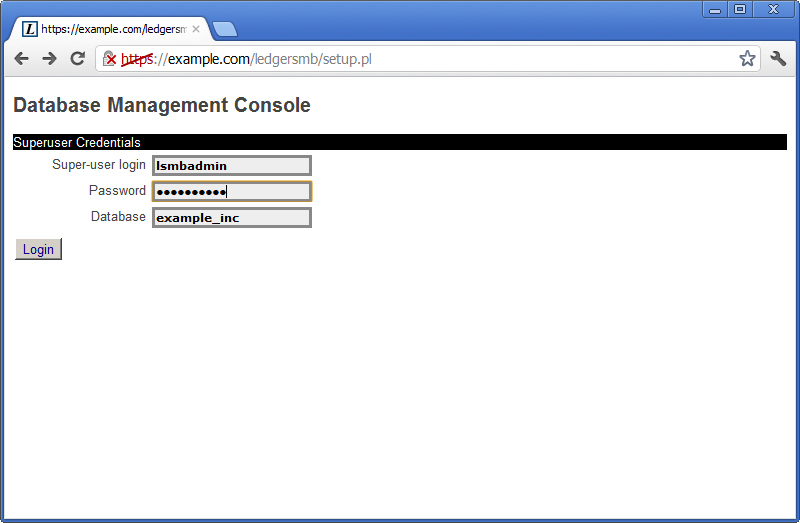
\includegraphics[width=0.8\textwidth]{dmc-create-step1.png}
\caption{setup.pl login screen}
\label{fig:setup-step1}
\end{figure}

\subsection{Step 2: Company creation}
\label{subsec-create-setup-create}

When creating a company database, there are a few things that are of importance:

\begin{itemize}
\item The name of the company database will be used at login time and hence
   will be used by all users - a choice of recognizable value is important
\item The value entered (and hence the company name) is case-sensitive
\item The name can't be more than 63 characters long
% \item ### others?
\end{itemize}

After choosing ``example\_inc'' as his company name, Jack clicks the Login button at which
time the screen from \figref{fig:setup-step2} shows up. The screen says the database doesn't yet exist and offers its creation.

\begin{figure}[h]
\centering
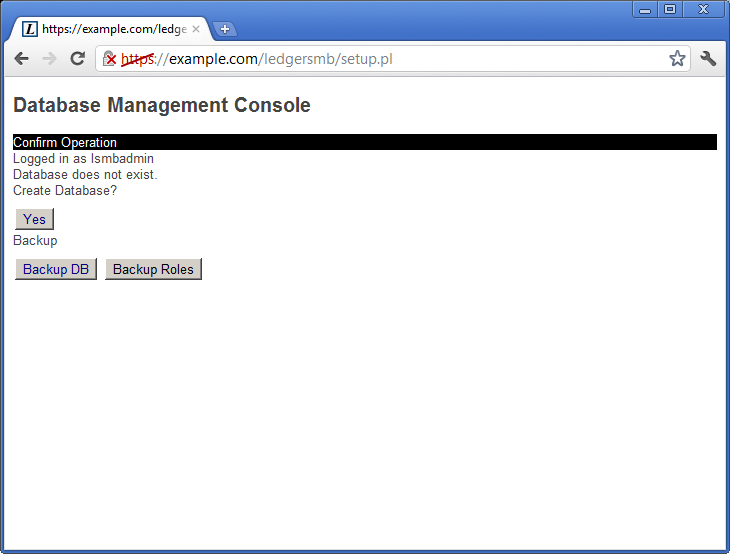
\includegraphics[width=7cm]{dmc-create-step2.png}
\caption{setup.pl company creation screen}
\label{fig:setup-step2}
\end{figure}

Jack clicks ``Yes'' to create the database and load it with LedgerSMB's database
schema, authorization rules and stored
procedures\footnote{Parts of the program inside the database.}. It may
take a while (30 seconds or more) for the next screen to appear\footnote{Note 
that during the creation of the database, logs are kept so that in case of
errors these can be reviewed either by the person running the installation or by
support personnel.  On Linux/Unix systems these are stored, by default, in
/tmp/ledgersmb/ and named dblog, dblog\_stderr and dblog\_stdout.}.

\subsection{Step 3: Selection of a Chart of Accounts}
\label{subsec-create-setup-select-coa}

LedgerSMB comes with numerous predefined charts of accounts\index{chart of accounts}. These have been grouped
per country making the selection of a chart a two-step procedure. setup.pl allows for
users wanting to define their own charts by offering a ``Skip'' button. This button
skips the process of loading a chart.

\begin{quote}
Note that you need to define a chart of accounts before you can meaningfully do anything
inside LedgerSMB. If you don't load a pre-defined one you'll need to create or upload
your own from inside the application once setup has completed.
\end{quote}

\figref{fig:setup-step3} shows the first screen in the \acrshort{CoA} selection procedure.
Here you select the country for which you want to use the \acrshort{CoA}. Note
that charts of accounts are highly country dependent and you may want to consult
an accountant if no default chart of accounts is included for your country.

As Jack runs his company in the United States, that's what he selects.

\begin{figure}[h]
\centering
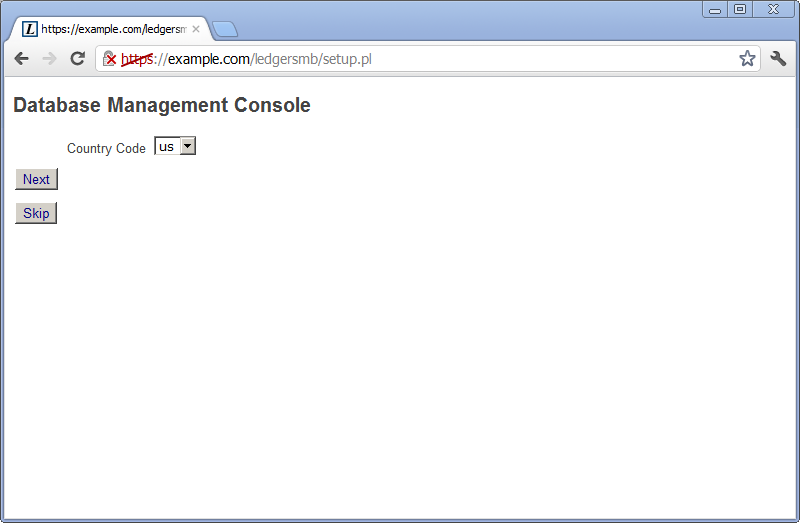
\includegraphics[width=7cm]{dmc-create-step3.png}
\caption{Chart of accounts - Country selection}
\label{fig:setup-step3}
\end{figure}

\figref{fig:setup-step4} shows the second screen in the chart of accounts selection procedure.
The drop down contains a list of all charts of accounts defined for the selected country.

Jack selects the \texttt{GeneralHierarchical.xml} chart of accounts: that will
leave him enough room to specialize the setup later if he has to, but for the time
being offers a broadly usable setup.

\begin{figure}[h]
\centering
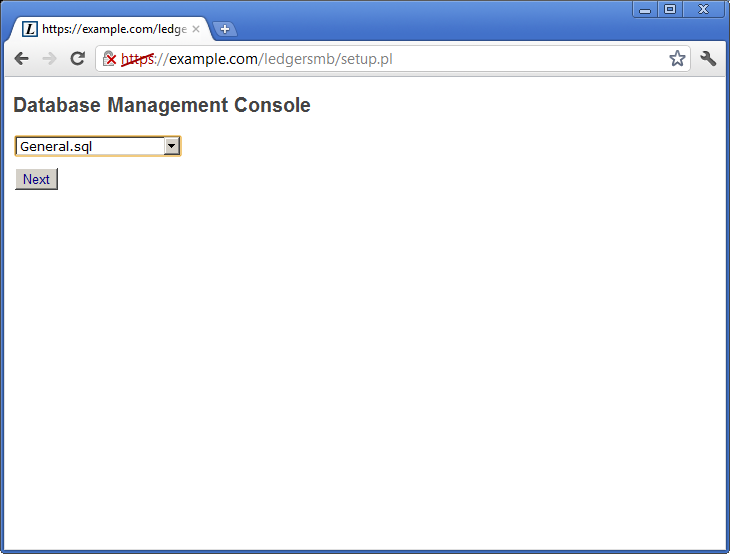
\includegraphics[width=7cm]{dmc-create-step4.png}
\caption{Chart of accounts - Chart selection}
\label{fig:setup-step4}
\end{figure}

\subsection{Step 4: Load template}
\label{subsec-create-setup-load-template}

LedgerSMB comes with a set of default reporting templates\index{templates}. 
These control the formatting of documents like invoices, checks, balance sheet, purchase orders, income statement, etc. 
Jack is now presented with the screen to load templates. LedgerSMB \ledgerSMBversion comes with a single choice\footnote{Administrators may define extra sets for users to be selected upon company creation; see \ref{sec-customization-company-creation-templates}}:
\begin{itemize}
        \item  \texttt{demo} -- Example template set for various output formats including PDF, HTML and Excel
\end{itemize}

\subsection{Step 5: Initial user}
\label{subsec-create-setup-initial-user}

In the previous step, the technical part of the company creation procedure
was completed. However, it's not possible to log in to the company yet. 
\figref{fig:setup-step5} shows the next step in the setup process:
 the user creation screen. The fields shown have
the same meaning as those discussed as part of user management in \secref{sec-user-creation}.

\begin{figure}[h]
\centering
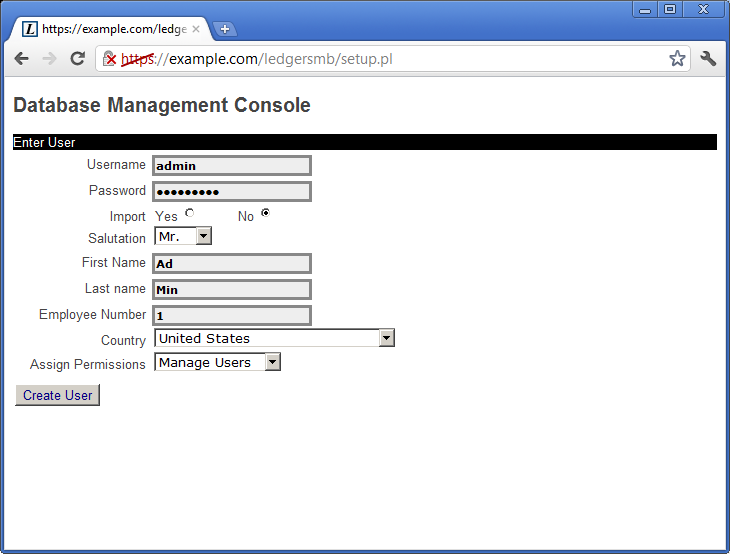
\includegraphics[width=7cm]{dmc-create-step5.png}
\caption{setup.pl initial user creation screen}
\label{fig:setup-step5}
\end{figure}

Jack chooses to create an administrative user called \texttt{admin} who will be authorized
to do everything in the application. Later on he will also create a user \texttt{jack}
who will be authorized to do everything but changing the configuration and doing application administration.
He'll use the latter user to log in for day to day operations. This will help him prevent changing settings by accident.

Note that none of the fields in this screen are optional. If the name of the user being created
isn't already used with other companies, leave the \texttt{Import} option set to \texttt{No},
otherwise please read the chapter on user creation mentioned above.

\begin{quotation}
Note: The password you enter here is a temporary one which will remain in effect
\textbf{for 24 hours only}. Be sure to execute the steps in \secref{sec-first-login-ramp-up} before
these 24 hours elapse, because the user will be disabled after that.
\end{quotation}

Jack proceeds to enter the values as follows:
\begin{longtable}{ llp{6cm} }
        Field & Value & Description \\ \hline
        \endhead
        User Name & \texttt{admin} & The login user name\\
        Password & \texttt{asdfg} & The password to use for your first login\\
        Create New User & \texttt{Checked} & \\
        Import Existing User & \texttt{Unchecked} & Only used when the user exists in another database\\
        Salutation & \texttt{Mr.} & \\
        First Name &  \texttt{Ad} & Used in combination with Last Name to identify the user \\
        Last Name & \texttt{Min} & \\
        Employee Number & \texttt{1} & \\
        Date of Birth & \texttt{1/1/2000} & not used by the application \\
        Tax ID/SSN & \texttt{0} & Tax or \acrshort{SSN}; not used by the application \\
        Country & \texttt{United States} & \\
        Assign Permissions & \texttt{Full Permissions} & \\
        \\
        \caption{Create first user entry data}
        \label{tbl:setupp-step5-user-entry-data}
\end{longtable}

@@@TODO: Replace figure below: it looks different these days (missing statistics section)
\begin{figure}[h]
\centering
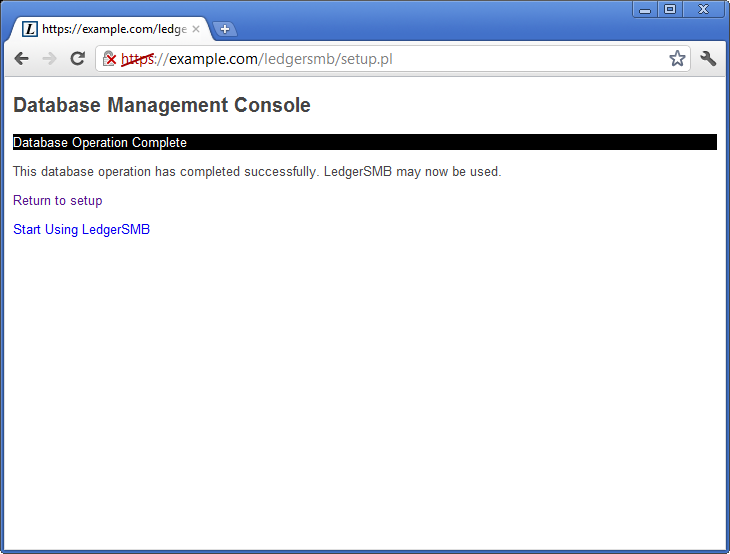
\includegraphics[width=7cm]{dmc-create-step6.png}
\caption{setup.pl successful completion screen}
\label{fig:setup-step6}
\end{figure}

Jack has created his company database and now sees the
 ``Database Management Console"  screen as shown in \figref{fig:setup-step6}.

By selection \texttt{Start using LedgerSMB} in the ``Database Operation Complete" section of the screen his story continues in
the next chapter ``The first login''.

\chapter{The first login}
\label{cha-first-login}

\section{Introduction}
\label{sec-first-login-introduction}

After the company database has been created by executing the procedure described in the last
chapter it is still an empty shell which needs to be populated. The correct data
needs to be entered for things like bank accounts and company contact data to be used
on invoices.

These steps have to be completed before LedgerSMB can be used meaningfully: these
settings have to be present for many workflows. A major reason is that with LedgerSMB
- as most \gls{erp} - financial
consequences of events in many workflows are directly reflected in the company's books.
Some accounting related settings have to be completed before LedgerSMB can do so.

This chapter documents the steps to create a basic usable configuration for Example Inc. 
It assumes that
one of the default chart of accounts was selected as shown in \charef{cha-company-creation} or 
that a custom chart of accounts was imported using the instructions in \secref{subsubsec-coa-importing}. 
Whatever method was chosen, this chapter assumes that a chart of accounts is available.

\section{Steps to the first login}
\label{sec-first-login-ramp-up}

Jack is ready for his first login and should see the screen as shown in \figref{fig:login-screen}.

If this screen is not shown then Jack navigates to 
\url{https://example.com/ledgersmb/login.pl} to access the login screen.

\subsection{Login screen}
\label{subsec-first-login-screen}

\begin{figure}[h]
\centering
% 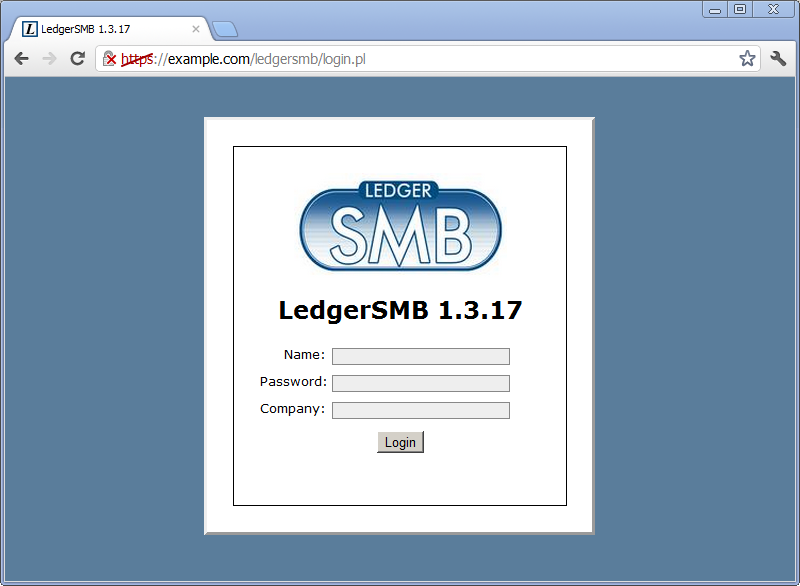
\includegraphics[width=7cm]{dmc-create-final.png}
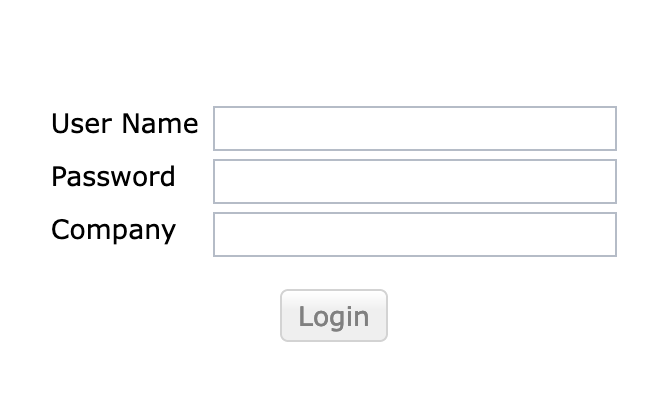
\includegraphics[width=9cm]{auto-screenshots/login.png}
\caption{login.pl opening screen}
\label{fig:login-screen}
\end{figure}

The login screen shows three fields which Jack proceeds to fill in as follows:

\begin{longtable}{ llp{6cm} }
        Field & Value & Description \\ \hline
        \endhead
        Name & \texttt{admin} & The login user name\\
        Password & \texttt{asdfg} & The password to use for your first login\\
        Company & \texttt{example\_inc} & The name of the company database \\
\end{longtable}

% \begin{description}
% \item[Name] The user name created during database setup; Jack uses \texttt{admin}
% \item[Password] The password - in this case for Jack's \texttt{admin} user
% \item[Company] The name of the database created; Jack uses \texttt{example\_inc}
% \end{description}

After entering all of the information and tapping the \texttt{Login} button Jack will see an alert letting
him know that his password will expire today.  Jack clicks \texttt{OK} to dismiss the alert.

\subsection{Selecting a password}
\label{subsec-first-login-password}

After successful login, the system shows the Welcome to LedgerSMB  screen as depicted in
\figref{fig:login-welcome-screen}.

\begin{figure}[h]
        \centering
        % \includegraphics[width=7cm]{welcome.png}
        \includegraphics[width=11cm]{auto-screenshots/welcome.png}
        \caption{login.pl welcome screen}
        \label{fig:login-welcome-screen}
\end{figure}

The
initial password has a 24-hour validity limit to prevent unused user accounts from posing
a security risk.  

To set a new password Jack navigates to \menupath{Preferences \ma Password} and sees the 
screen as depicted in \figref{fig:first-user-password}.

The new password that Jack chooses will be different than any password used before and 
different than the temporary password set by the administrator.
Not clicking the \texttt{Save} button means the password remains unchanged and the
24-hour limit remains in effect.

\begin{figure}[H]
\centering
% 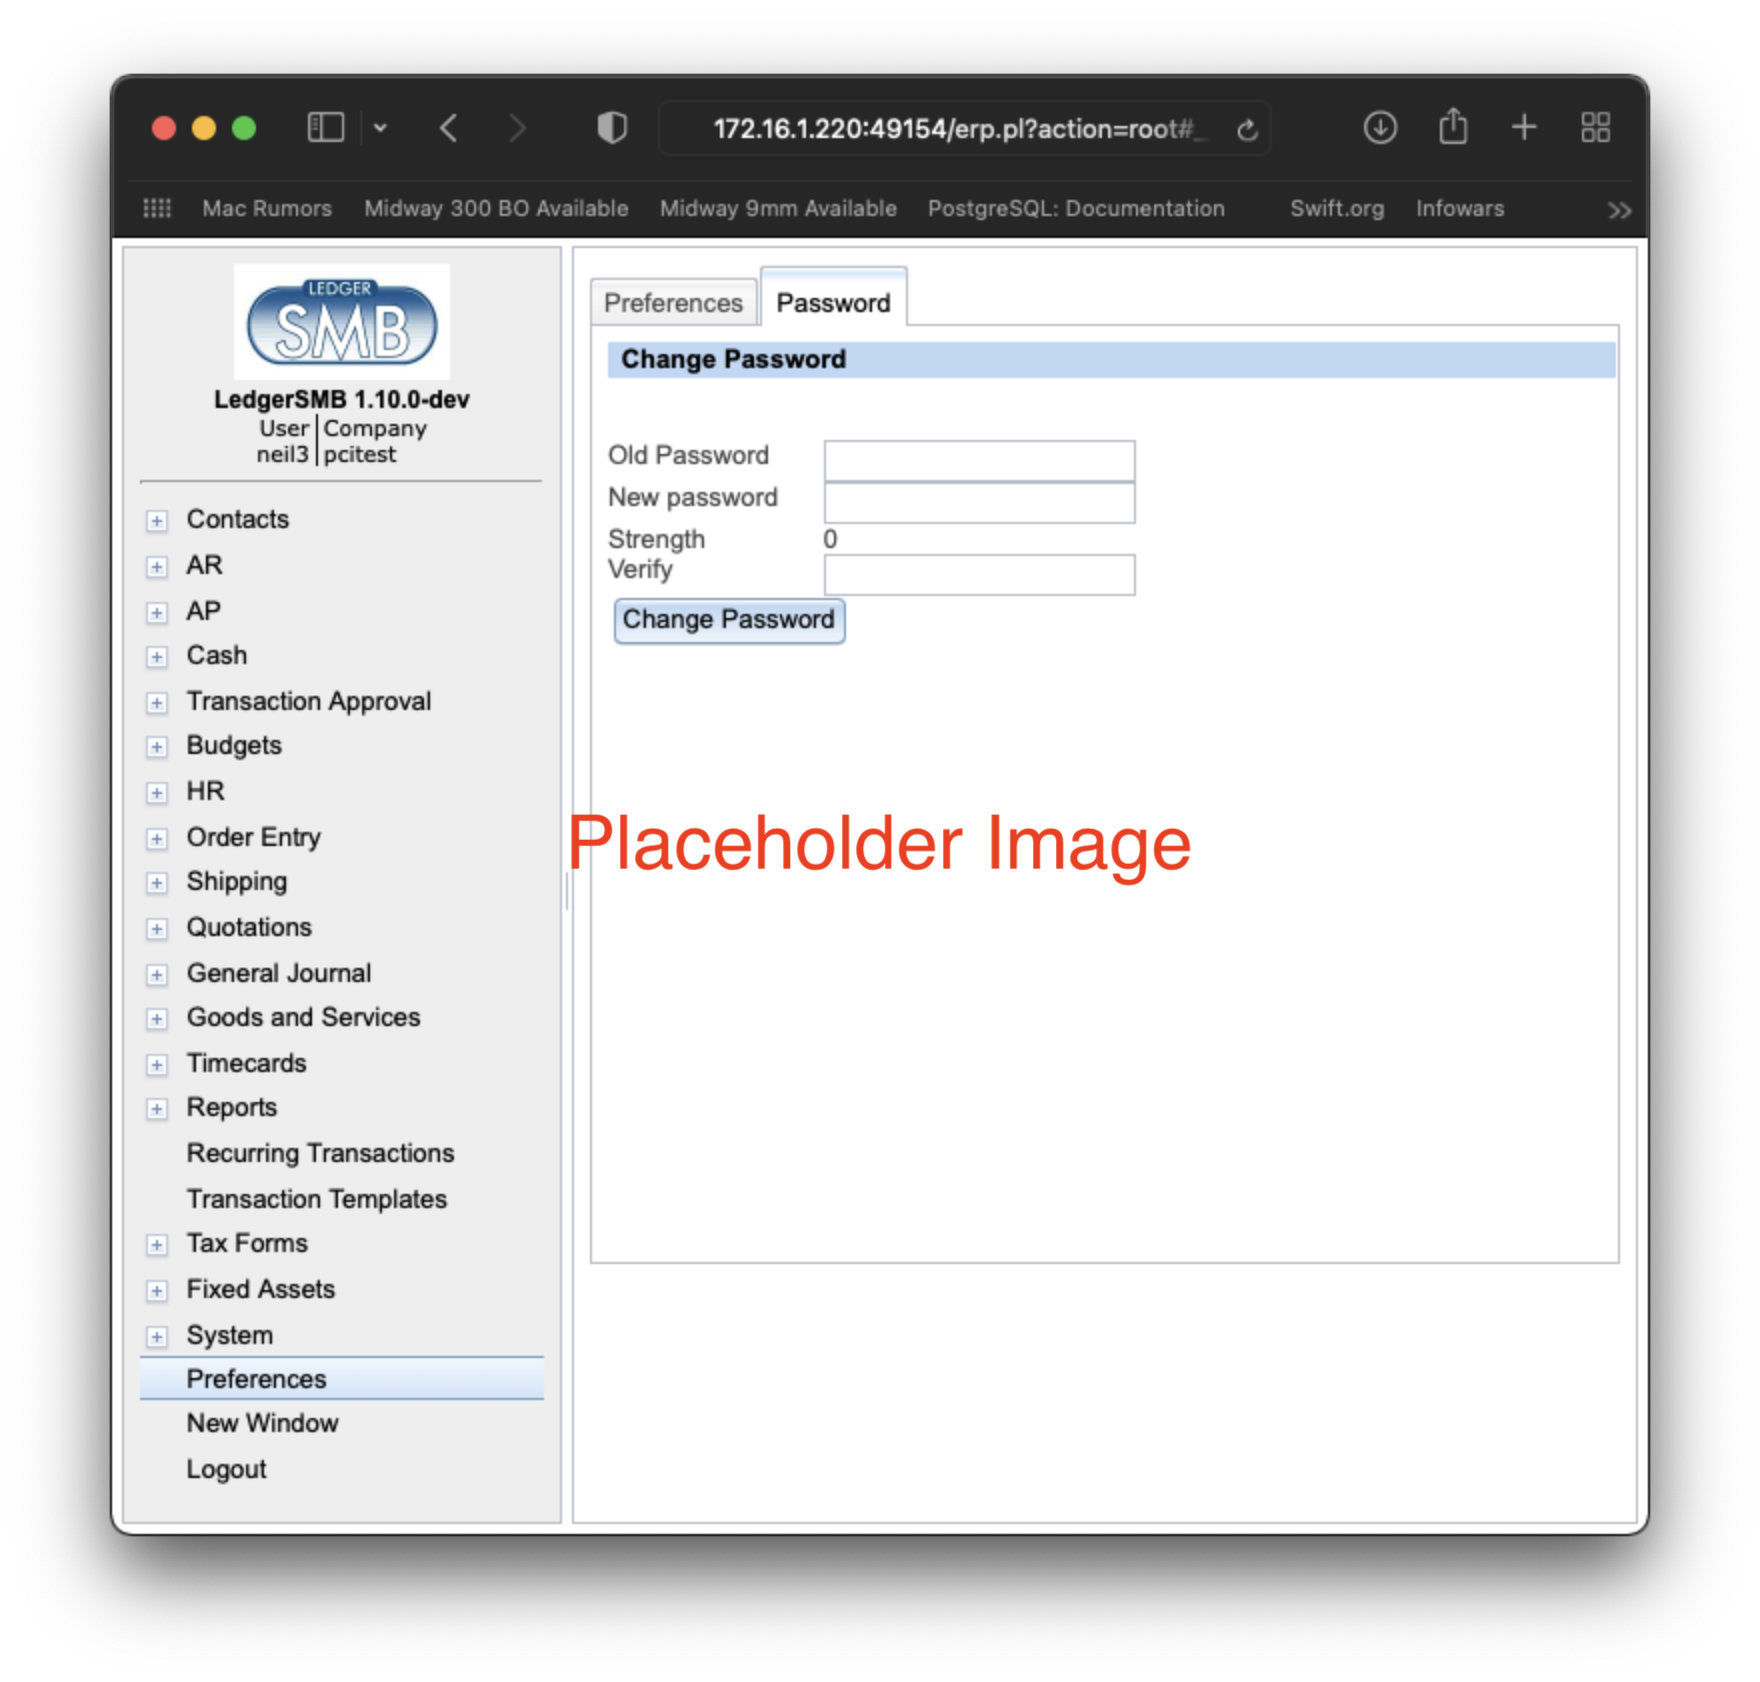
\includegraphics[width=7cm]{user-password.png}
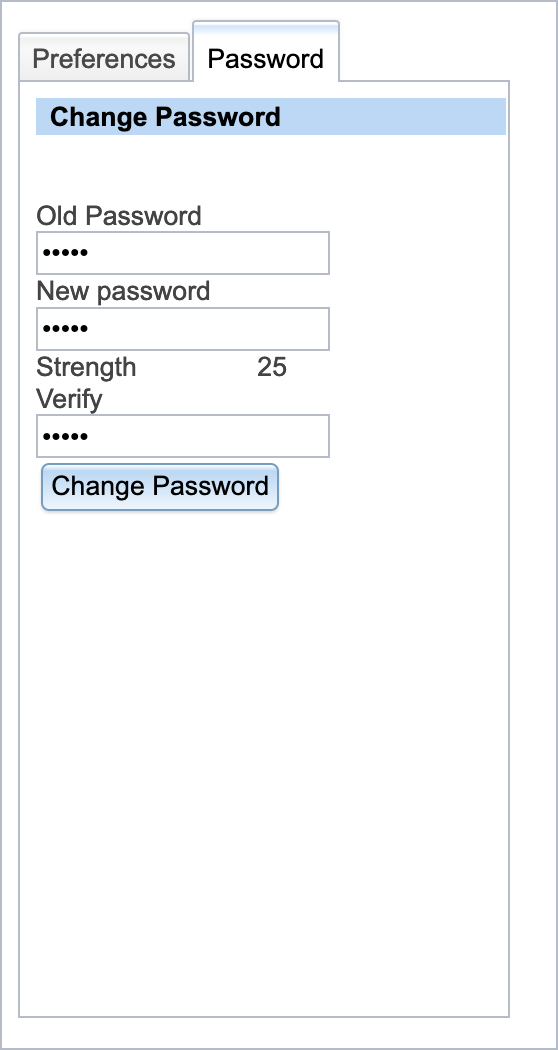
\includegraphics[width=11cm, trim={3pt 300 2 4}, clip]{auto-screenshots/preferences-password.png}
\caption{Password change screen}
\label{fig:first-user-password}
\end{figure}

Jack enters the information in the Change Password screen as follows:
\begin{longtable}{ llp{6cm} }
        Field & Value & Description \\ \hline
        \endhead
        Old Password & \texttt{asdfg} & The old password set by the administrator using setup.pl\\
        New Password & \texttt{lkjhg} & The new password that Jack wants to use for admin\\
        Verify & \texttt{lkjhg} &  Repeats the new password that Jack wants to use for admin\\
        \\
        \caption{First Login - Change initial password data}
        \label{fig:first-user-change-initial-password}
\end{longtable}

%\begin{description}
%       \item[Old Password] The old password originally set by the administrator using \texttt{setup.pl}
%       \item[New Password] The new password for Jack's account.
%       \item[Verify] The new password for Jack's account.
%\end{description}

Jack then clicks the \texttt{Change Password} button.

The new password has a validity of determined by the \texttt{Password Duration} setting
from the \menupath{System \ma Defaults} screen. User management is discussed is detail in \charef{cha-user-management}.

Login will be denied to users with expired passwords; they can request
password resets through user admins.

\subsection{Setting user preferences}
\label{subsec-setting-user-preferences}

Jack clicks on the tab \texttt{Preferences} and the system shows the Preferences screen 
as depicted in \figref{fig:user-preferences}

\begin{figure}[H]
        \centering
        %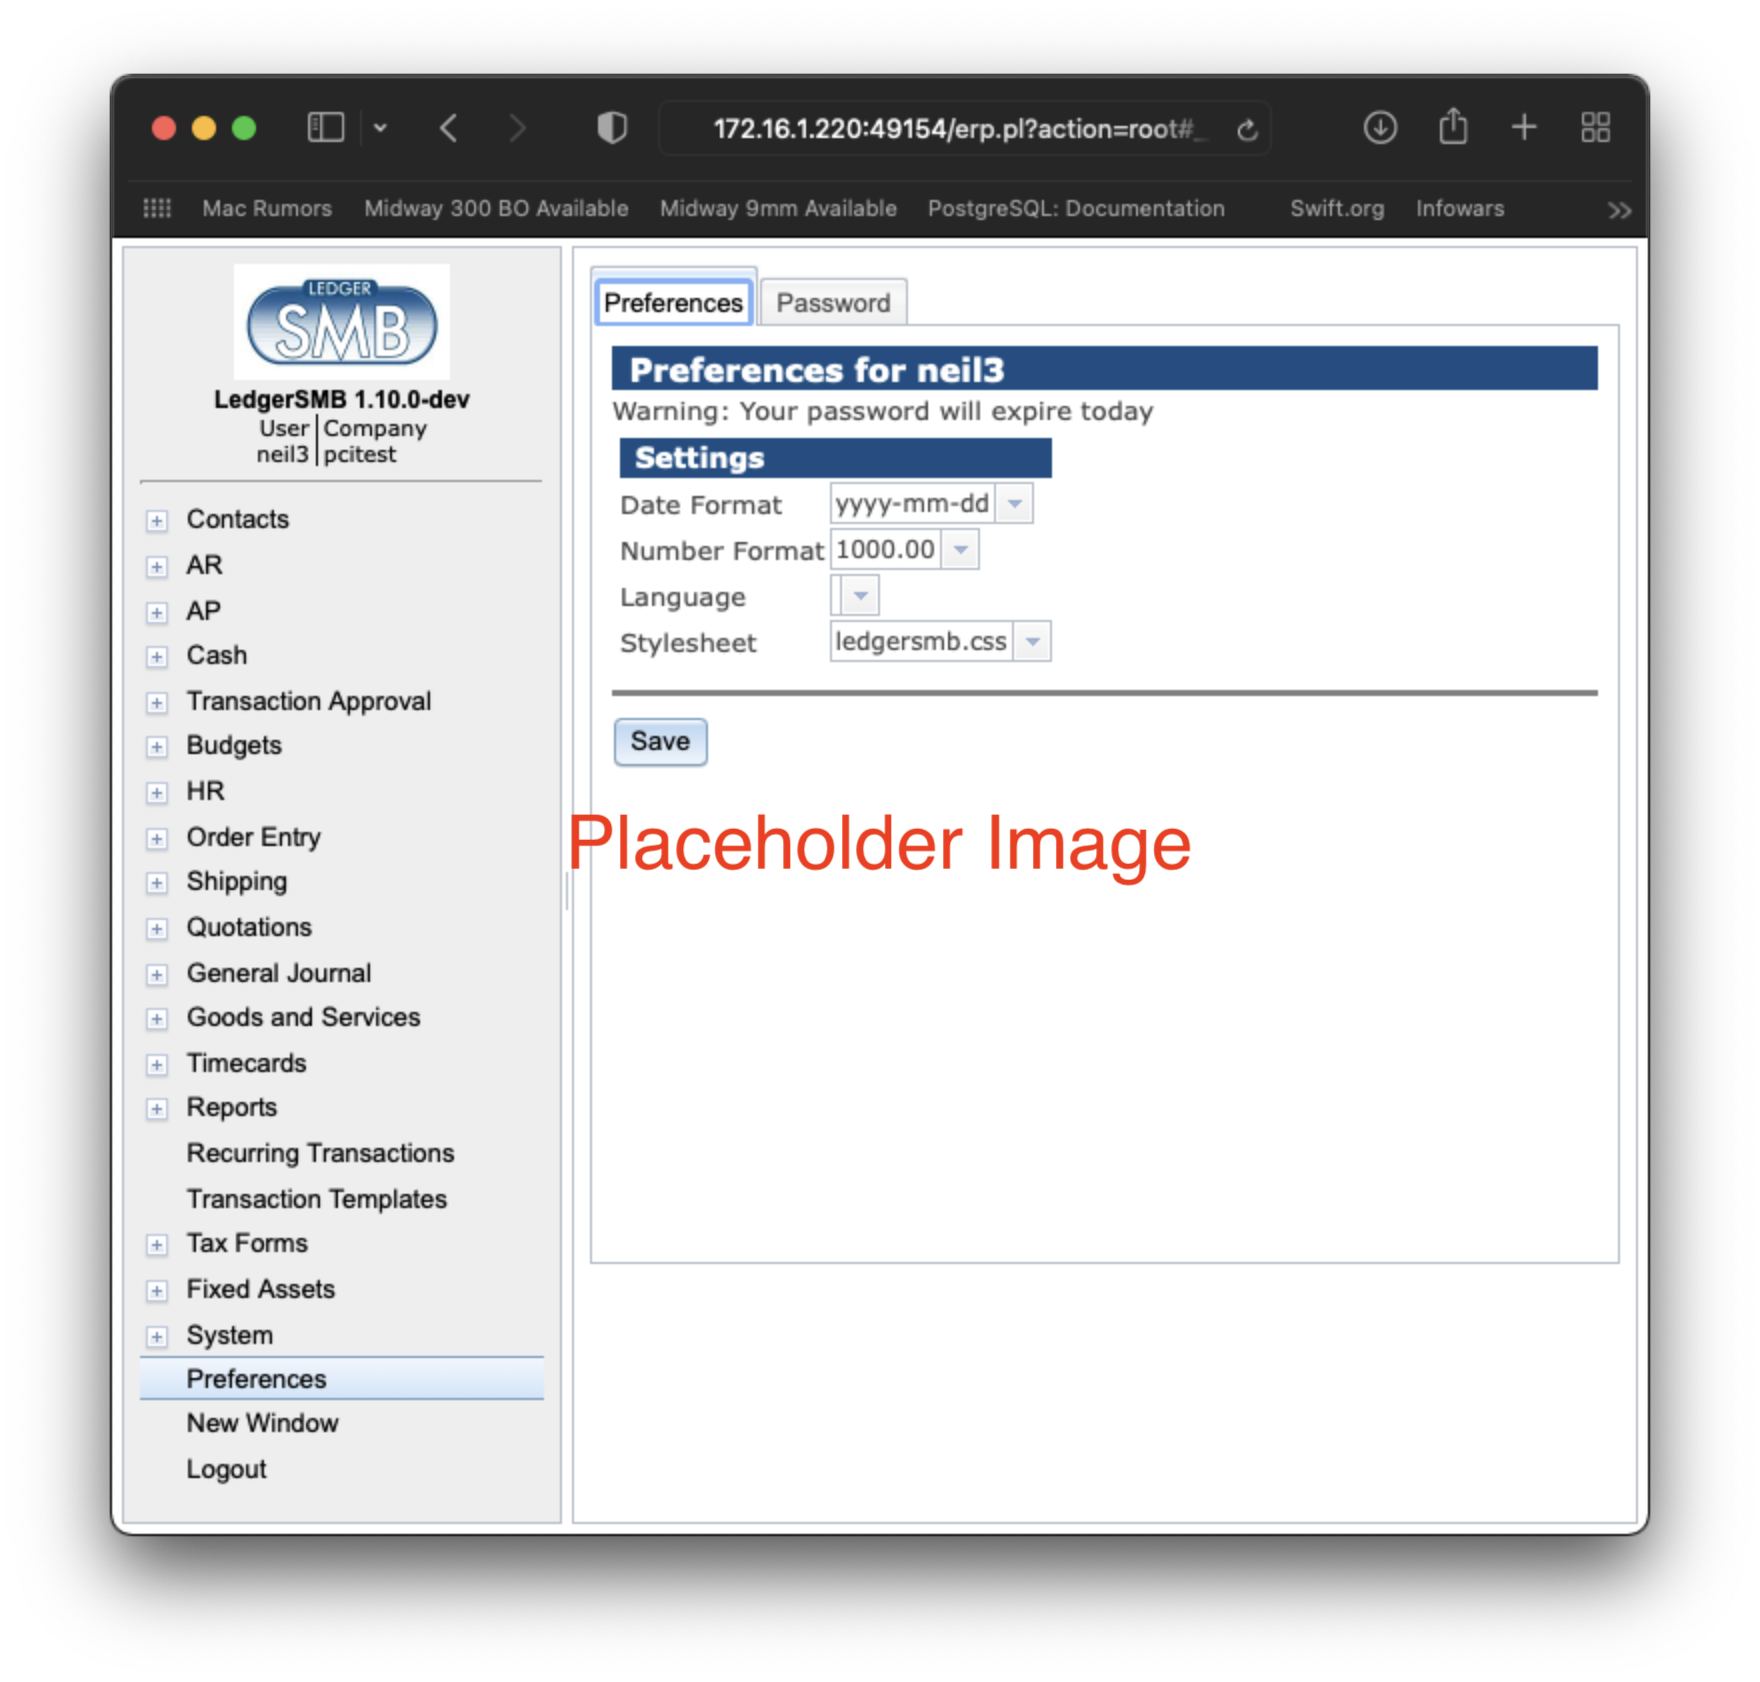
\includegraphics[width=7cm]{user-preferences.png}
        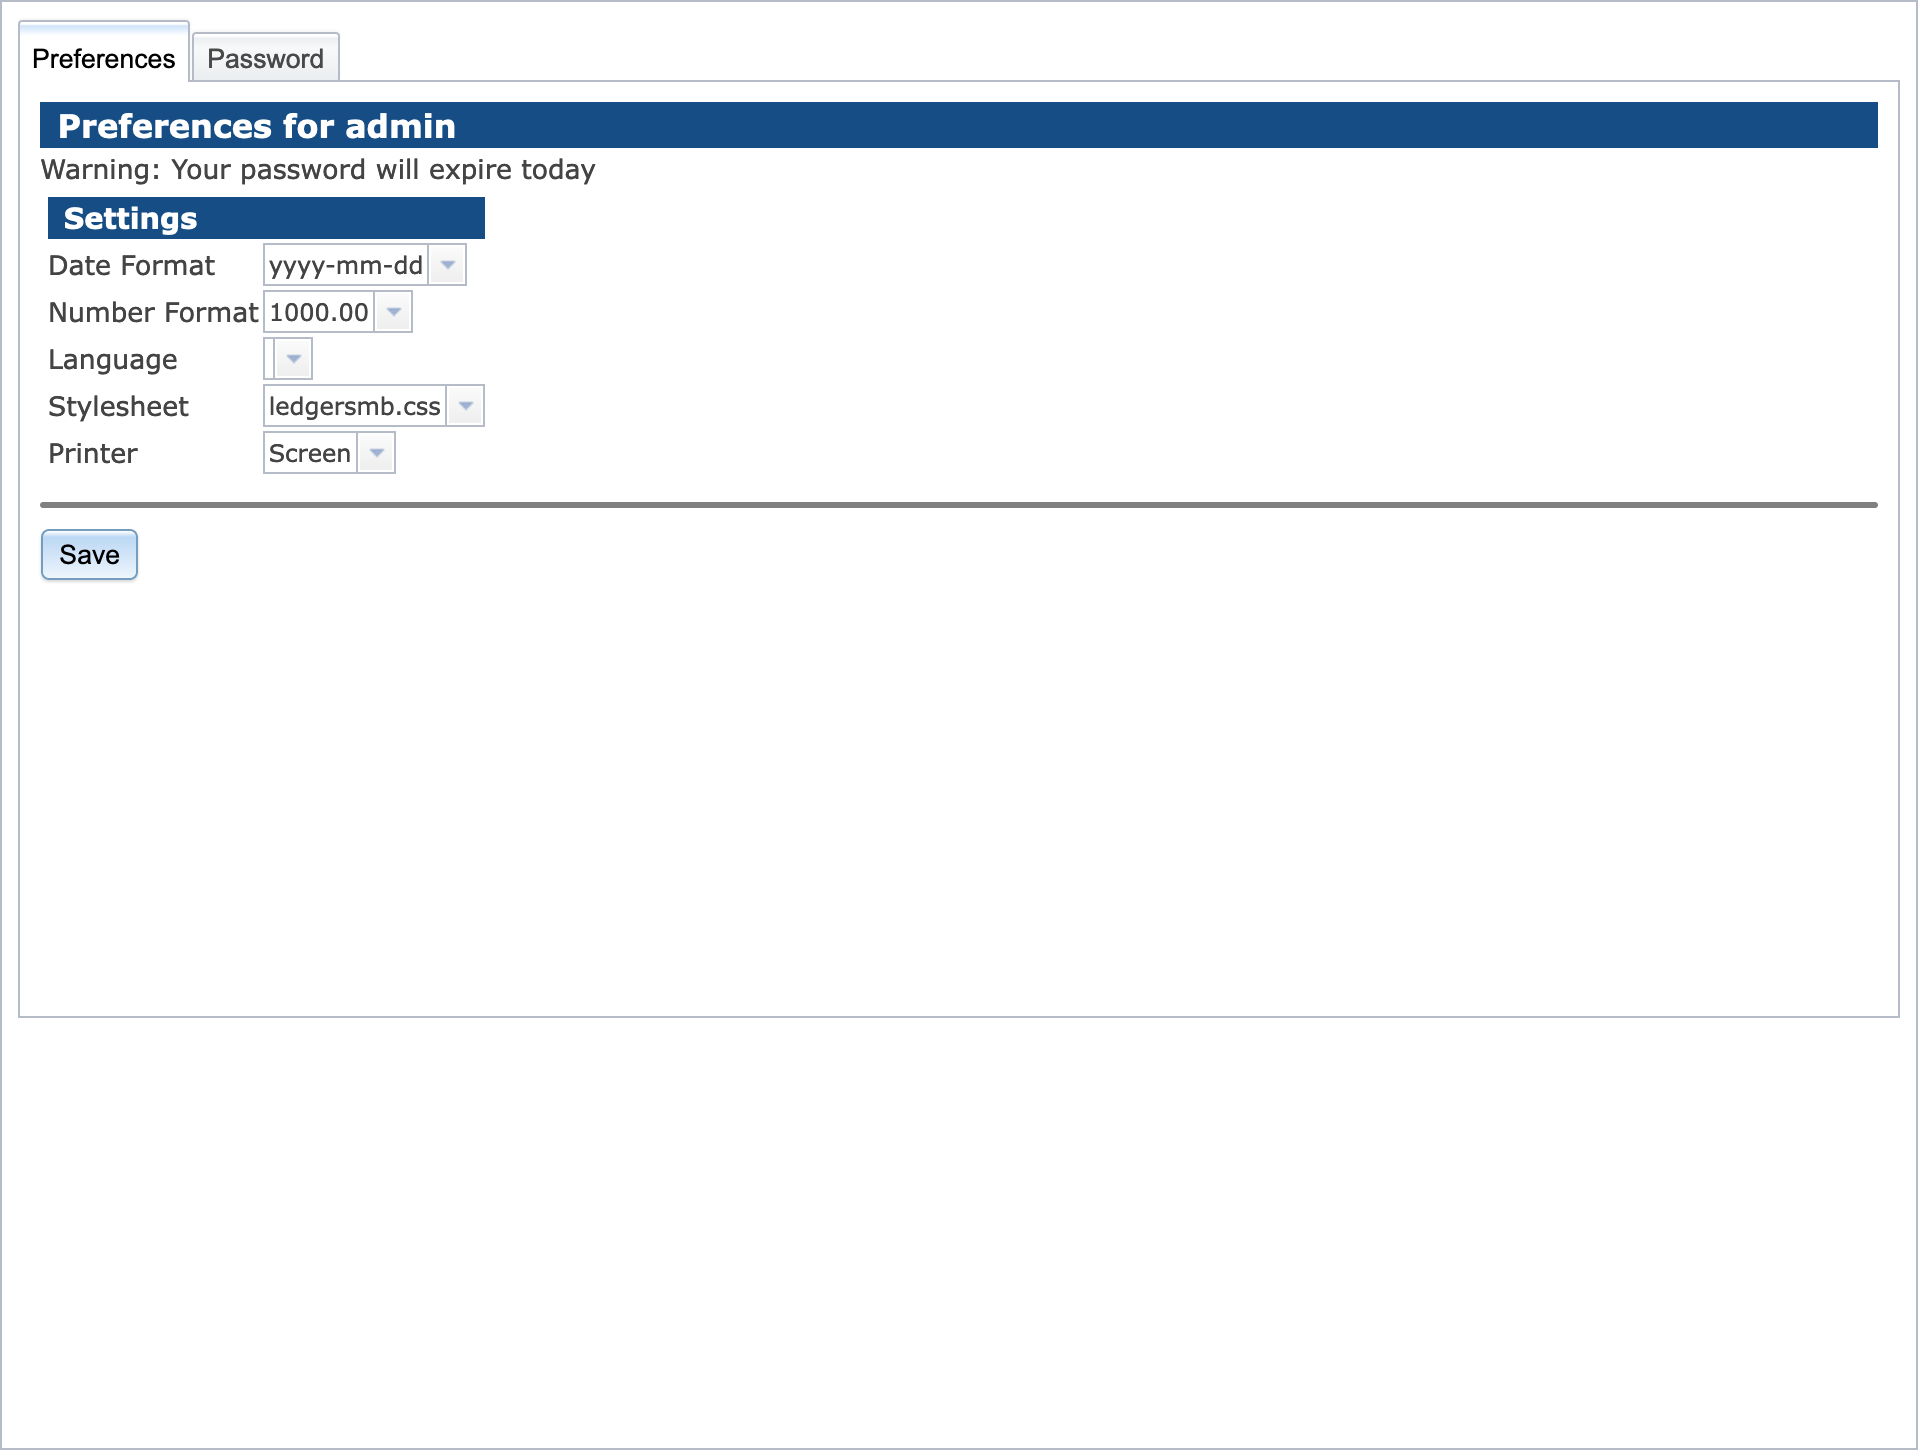
\includegraphics[width=11cm]{auto-screenshots/preferences-preferences.png}
        \caption{User preferences}
        \label{fig:first-user-preferences}
\end{figure}

Jack selects his language, in this case \texttt{American English} and clicks \texttt{Save}.

\subsection{Setting system defaults}
\label{subsec-setting-system-defaults}

Out of the box, LedgerSMB contains reasonable system defaults, but Jack needs to add some specific company information.
In order to do so, Jack navigates to \menupath{System \ma Defaults} and sees the screen depicted in \figref{fig:first-user-system-defaults}.

\begin{figure}[H]
        \centering
        % 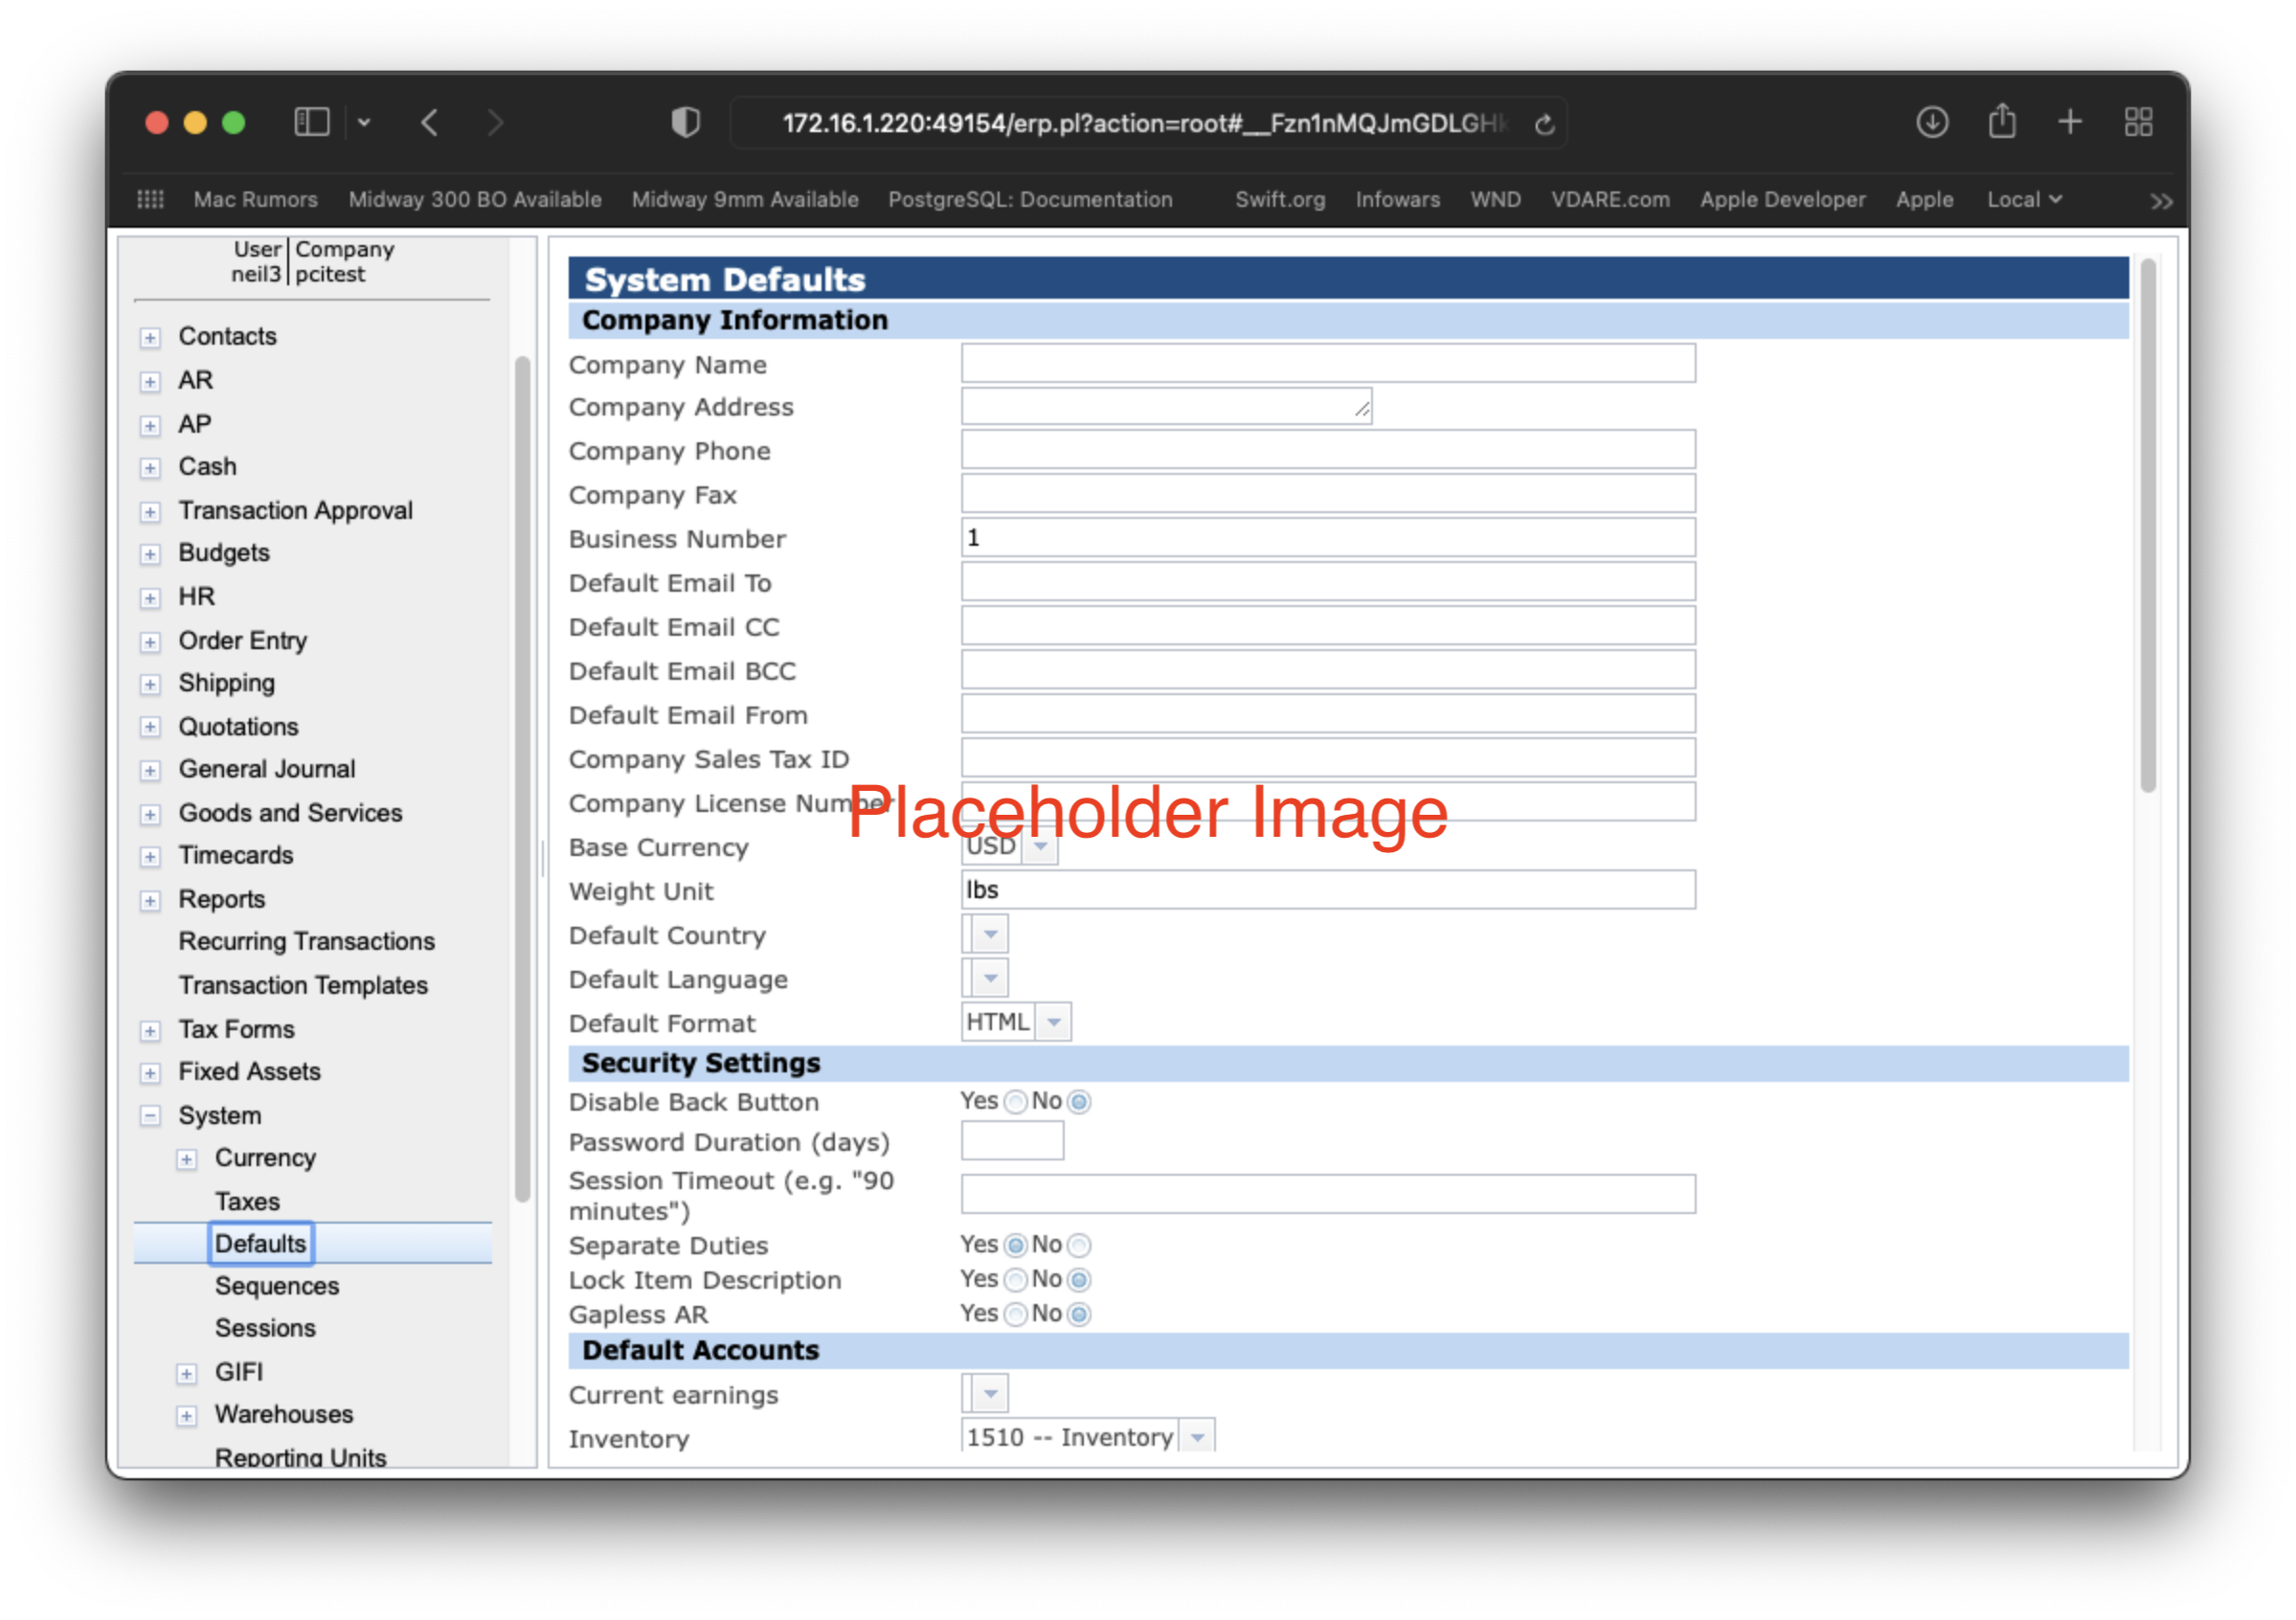
\includegraphics[width=7cm]{system-defaults.png}
        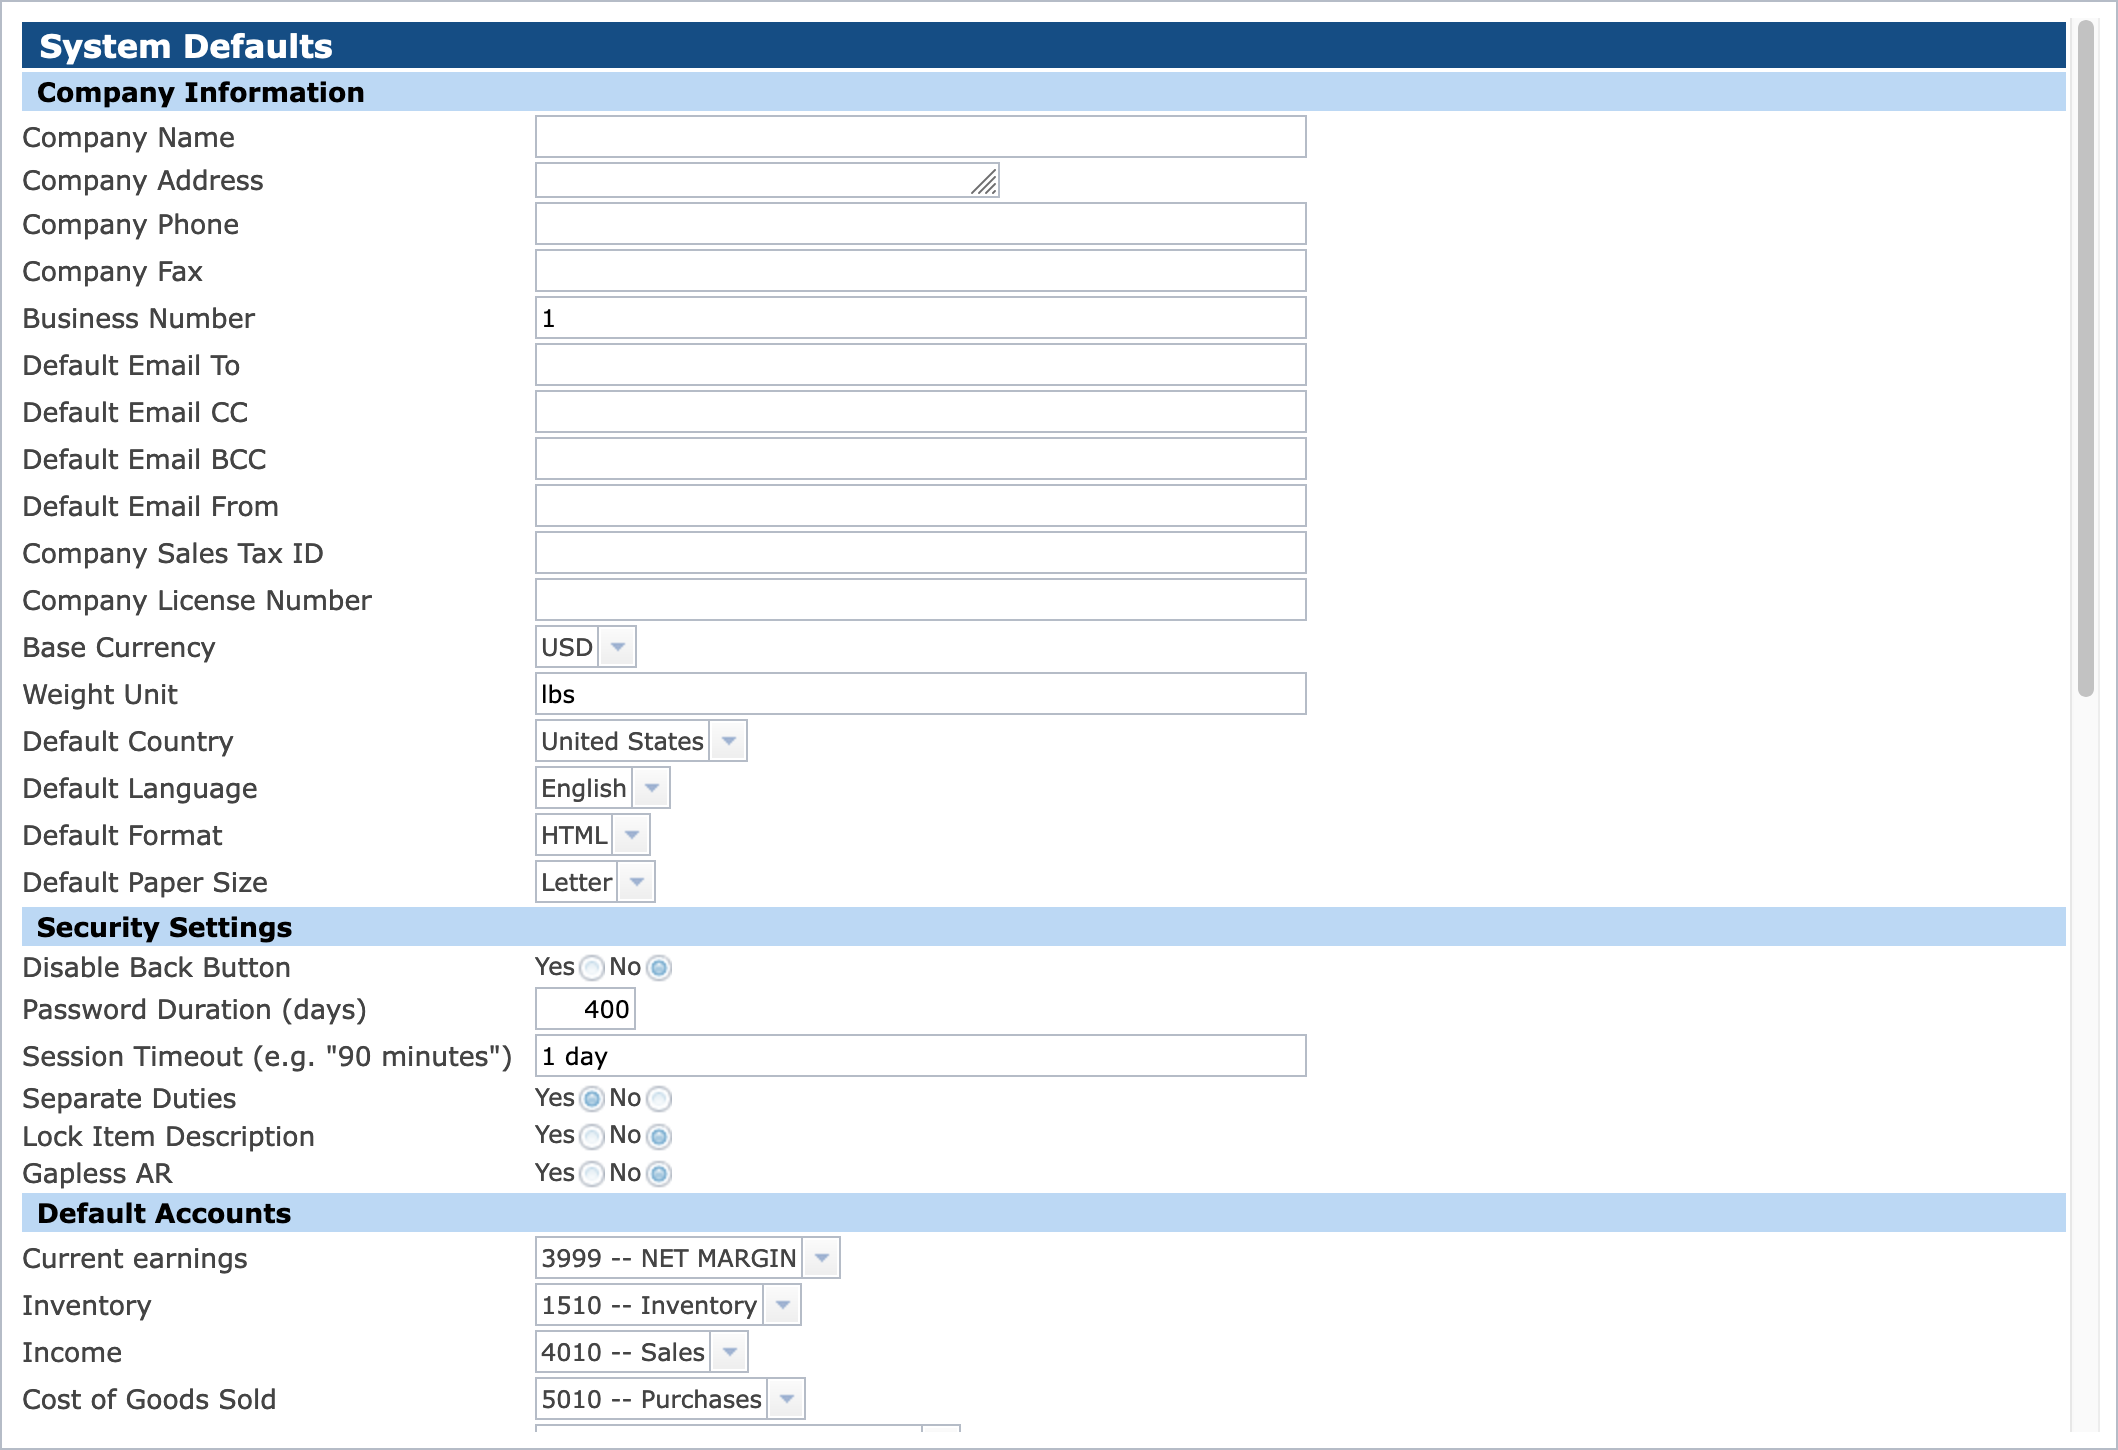
\includegraphics[width=11cm]{auto-screenshots/system--defaults.png}
        \caption{System defaults}
        \label{fig:first-user-system-defaults}
\end{figure}

Jack sets the following defaults:
\begin{longtable}{ llp{6cm} }
        Field & Value & Description \\ \hline
        \endhead
        Company Name & \texttt{Example Inc.} & \\
        Company Address &  \makecell[l]{\texttt{215 Example St} \\  \texttt{Any City, CA}} & Note the use of the new line\\
        Company Phone &  \texttt{555 836 2255} & \\
        Business Number &  \texttt{12345} & e.g. Chamber of commerce number\\
        Default Email From & \texttt{info@example.com} & \\
        Default Country & \texttt{United States}  & \\
        Default Language &  \texttt{English (US)} & \\
        Password Duration &  \texttt{180} & Days\\
        \\
\caption{First Login - Change user defaults data}
\label{fig:first-user-user-default-data}
\end{longtable}

%\begin{itemize}
%       \item \textbf{Company Name} to \texttt{Example Inc.}
%       \item \textbf{Company Address} to  \texttt{215 Example street, Any City, CA}
%       \item \textbf{Company Phone} to \texttt{555 836 2255}
%       \item \textbf{Business Number} (e.g. Chamber of commerce number) to \texttt{12345}
%       \item \textbf{Default Email From} to \texttt{info@example.com}
%       \item \textbf{Default Country} to \texttt{United States} 
%       \item \textbf{Default Language} to \texttt{English (US)}
%       \item \textbf{Password Duration} to \texttt{180}
%\end{itemize}

A more elaborate description of the parameters in this screen is provided in subsection
\ref{subsec-company-config-defaults}.

\section{Setting up a bank account or credit card}
\label{sec-first-login-setup-bank-account}

As part of the start up activities of his company, Jack comes to an agreement with the
bank for three products:

\begin{itemize}
\item A current account with number ``C54769''
\item Deposit account with number ``D54990''
\item Credit card with a number ending with ``.7734''
\end{itemize}

Most accounting systems - LedgerSMB included - use separate GL accounts to represent
each bank account. This allows easy reconciliation of the ending balance on the bank
account with the balance in the books.

Knowing this, Jack looks up the example bank account from his preconfigured US chart of
accounts using the \menupath{General Journal \ma Chart of Accounts} menu as
shown in \figref{fig:bank-setup1}.

\begin{figure}[h]
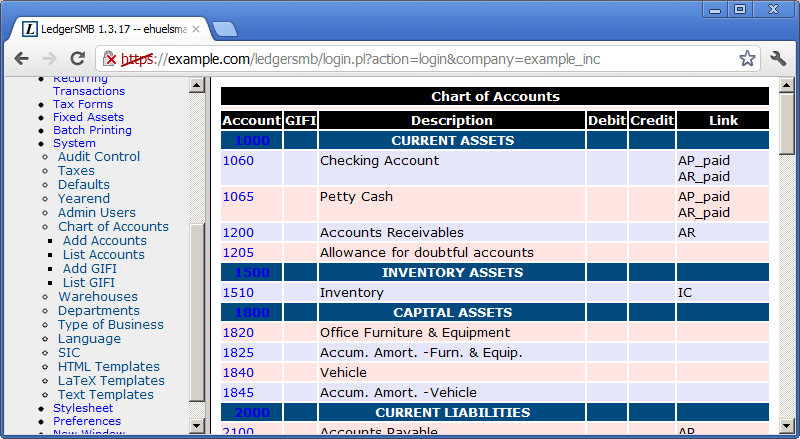
\includegraphics[width=\linewidth]{setup-bank-account1.png}
\caption{Bank account setup - menu items}
\label{fig:bank-setup1}
\end{figure}

Jack adds the new bank accounts by doing the following:

\begin{enumerate}
\item Click on ``1060''
\item The screen appears as shown in \figref{fig:bank-setup2} appears 
\item Change the Description ``Checking Account'' to ``Checking Account C54769''
\item Click ``Save''
\item In the same screen change the Account Number to ``1061''
\item Change the Description to ``Cash Deposit Account D54990''
\item Click ``Save as new''
\item In the same screen change the Account Number to ``1062""
\item Change the description to ``Credit Card xxxx.xxxx.7734''
\item Click ``Save as new''
\end{enumerate}

\secref{sec-coa-account-options} discusses the options in detail - for now using the
settings as configured for the sample checking account will do.

\begin{figure}[h]
        \centering
% 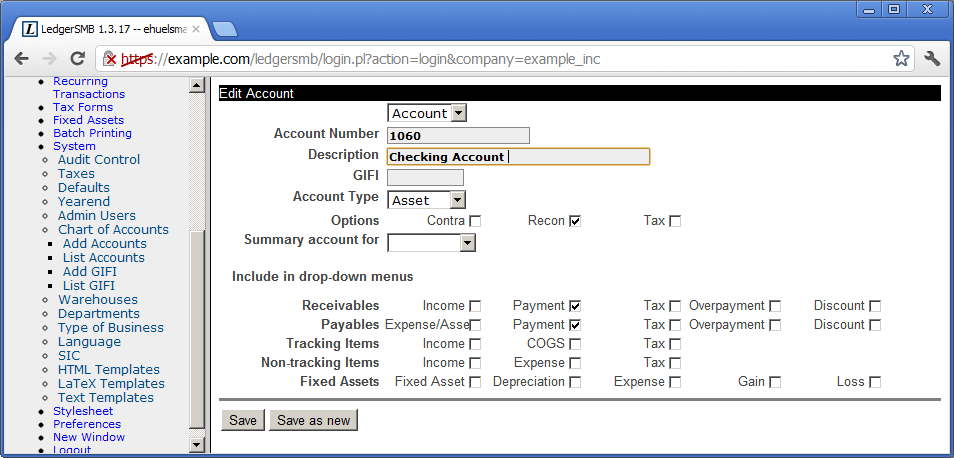
\includegraphics[width=\linewidth]{setup-bank-account2.png}
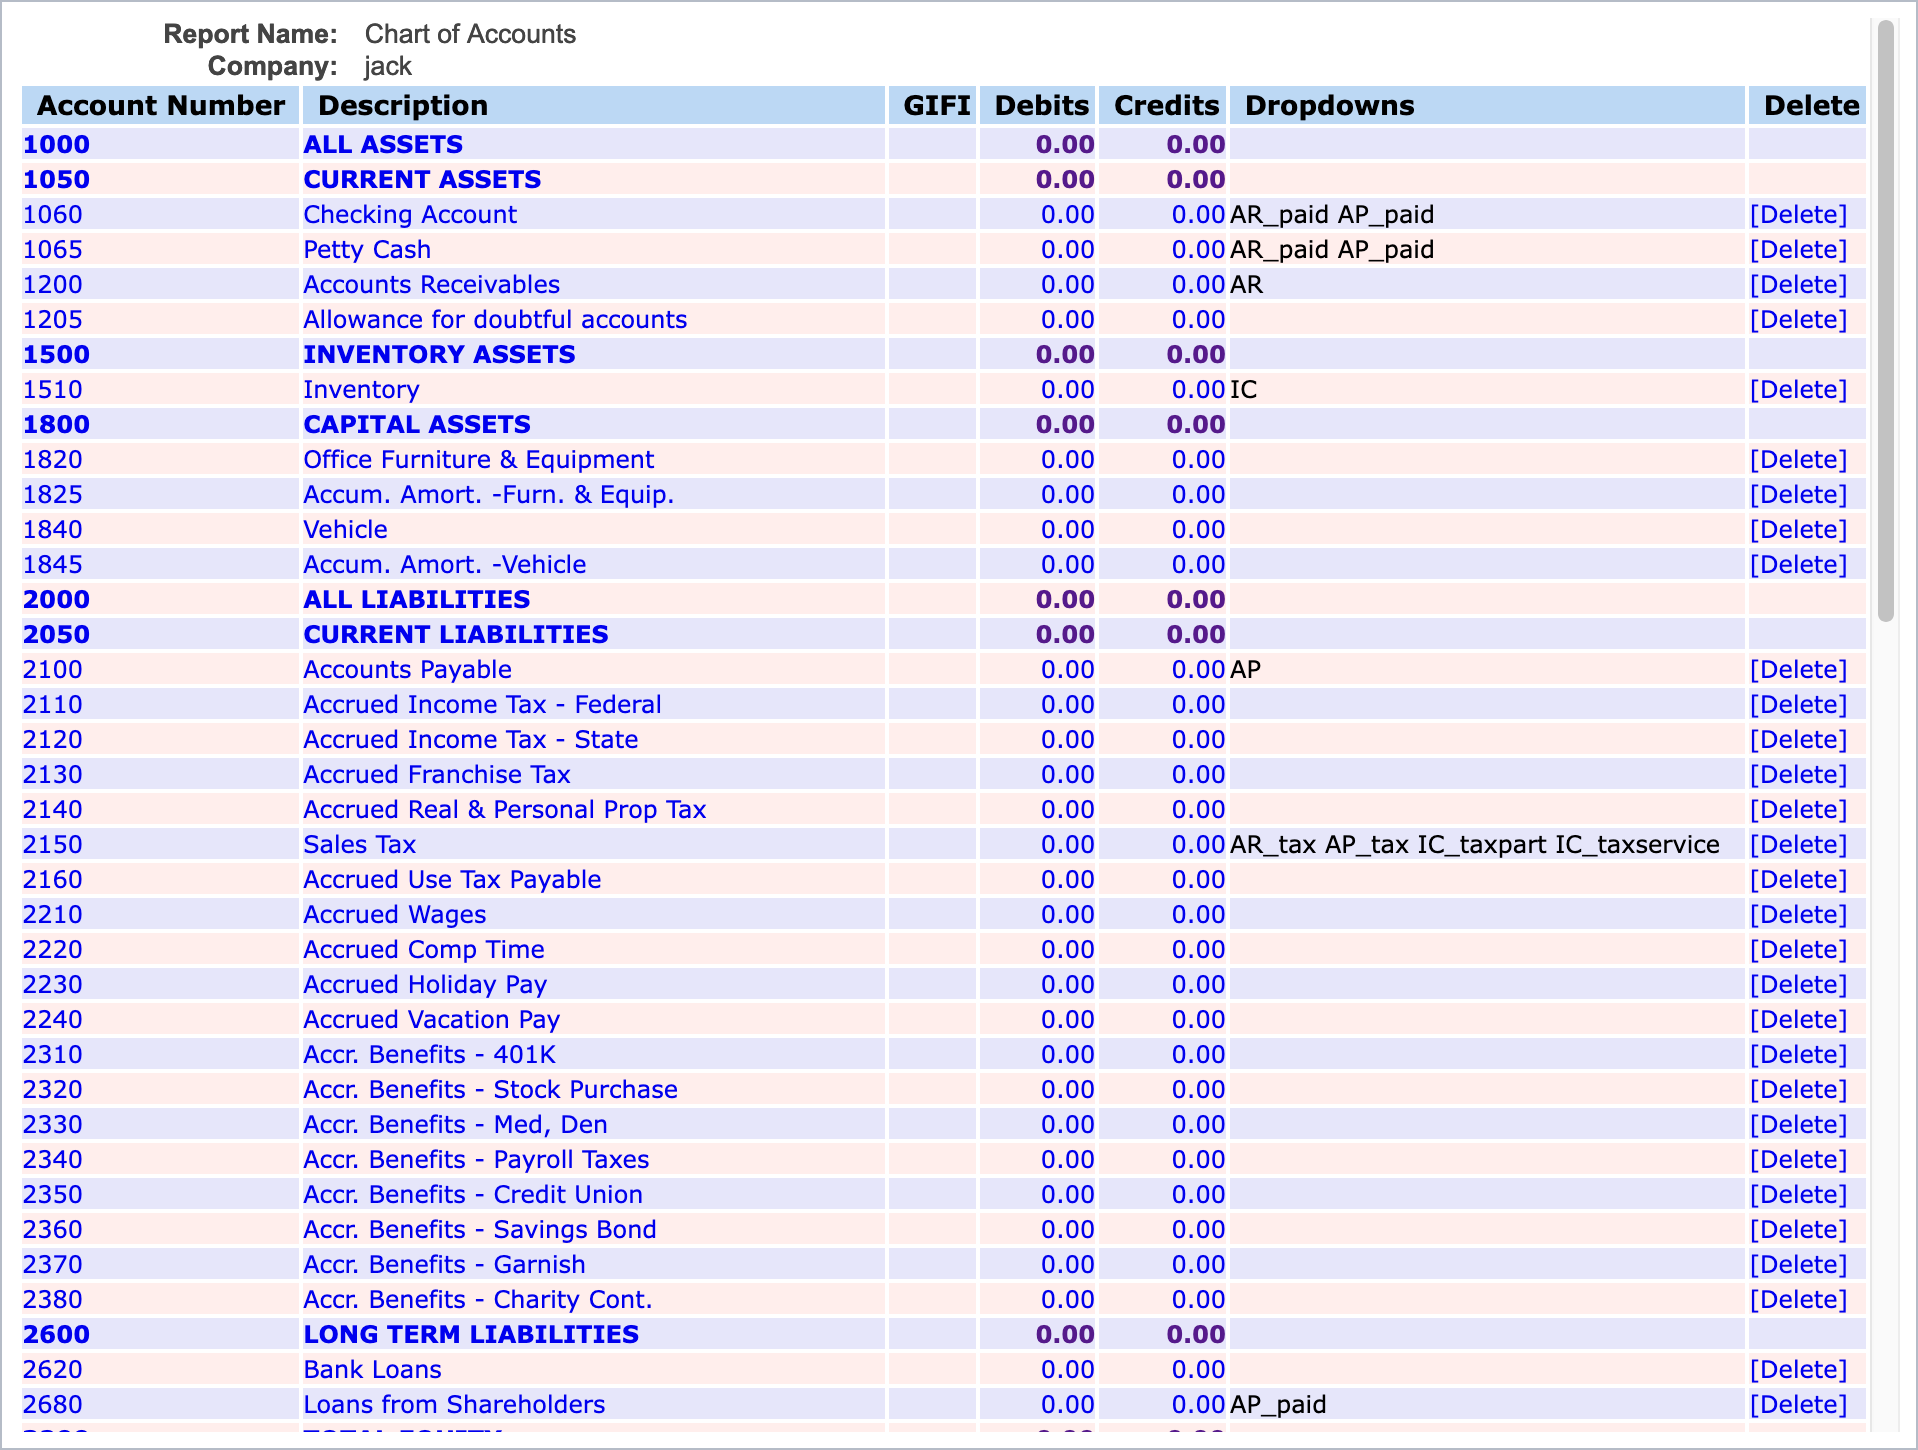
\includegraphics[width=11cm]{auto-screenshots/general-journal--chart-of-accounts.png}
\caption{Bank account setup - account setup screen}
\label{fig:bank-setup2}
\end{figure}


\section{Checking and adjusting the chart of accounts}
\label{sec-first-login-coa-check}

First and foremost the chart of accounts serves to register income, expenses,
assets and liabilities in categories which support financial decision making or
regulatory requirements. When checking his chart of accounts, this is the first
thing Jack checks for.

Many business events in LedgerSMB trigger the creation of financial transactions.
If the configuration required for these transactions to be created isn't in place,
users won't be able to complete their workflows. 

\subsection{Accounts list}
\label{subsec-first-login-accounts-list}

Jack wants to make sure his chart of accounts fits his purposes. To perform these
checks Jack goes into the \menupath{General Journal \ma Chart of Accounts} page. For now, he finds
the ledger to be in order. Although the single Sales account stands out a bit against
the numerous expense accounts, it turns out that there is also a single Purchases
account on which all the expenses for parts purchases are going to be booked.

He decides that if this isn't enough, he can add accounts later.
\footnote{Note that Jack will discover in \secref{sec-stock-defining-vendors} that
he does indeed need to create additional accounts to support sales and
purchase discounts.}


\section{Checking sales tax rates}
\label{sec-first-login-checking-tax-rates}

First off, Jack asserts that a sales tax\footnote{Sales tax may be called \gls{VAT}
in some jurisdictions.} account has been provisioned. He finds it
in the Current Liabilities section of his \gls{CoA}. In his jurisdiction there
is only one sales tax rate applicable at any one time, which means this single account
will suit his needs just fine. If he had been in a jurisdiction with multiple tax rates
applicable, e.g. different rates for different types of goods, he would have been
required to create more accounts.

The procedure to create more sales tax accounts is the same as the one used in
\secref{sec-first-login-setup-bank-account}, with the notable difference that this time the base account
to be used is the sales tax account.

With the accounts in place, the tax rates have to be checked and possibly adjusted.
To do so, Jack navigates to the \menupath{System \ma Taxes} page as shown in \figref{fig:setup-tax-rates}.

\begin{figure}[h]
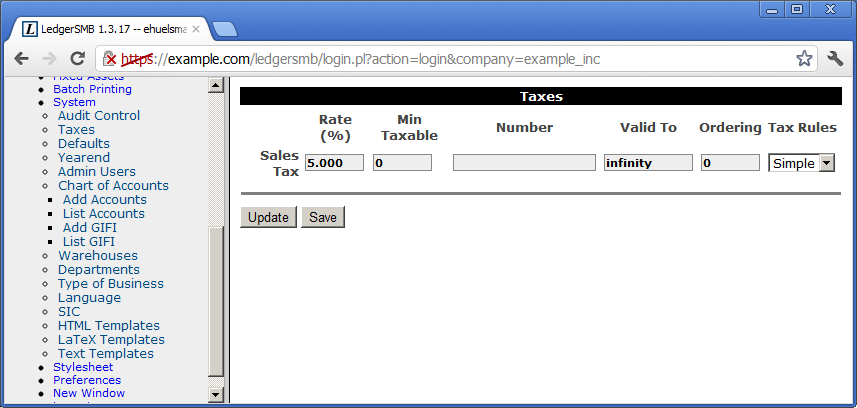
\includegraphics[width=\linewidth]{setup-tax-rates.png}
\caption{Tax rate adjustment screen}
\label{fig:setup-tax-rates}
\end{figure}

The rate shown (5\%) is exactly what Jack needs. The procedure to set rates is a bit
long to describe and hence has its own chapter. Please refer to \charef{cha-taxes} for
details on how to change taxes.

\chapter{Building up stock}
\label{cha-building-up-stock}

\section{Overview}
\label{sec-stock-overview}

In this chapter Jack goes through the process of setting up LedgerSMB for his
trade activities in computer parts, which includes deciding which parts he wants to
resell. From there on he goes to contact a vendor to request a quotation, convert that
to an order and receive goods into inventory and invoices into accounts payable.

To prepare LedgerSMB for his parts sales and purchases, Jack needs to configure Parts.
The system records inventory for parts and assemblies. Jack won't use them for his
business. There's more on assemblies in \secref{subsec-assemblies-definition}.

Once set up, Jack is ready to execute the ordering process. Even though the process
is described here from a purchasing perspective, sales work the same way with the roles
reversed (Jack will act as a vendor in the sales process).

To start his purchase, Jack creates a \gls{rfq} document which
he sends one or multiple vendors to let them know he's interested in their products.

The vendor responds to Jack's request by issuing a Quotation. From a legal perspective
a quotation is a document which promises to deliver the requested goods or services at a
certain rate - subject to conditions specifically mentioned. If Jack accepts the quotation
and meets the conditions, the vendor is obligated to deliver.

In response to the quotation, Jack will place an order with the vendor to indicate
acceptance of the quotation (or he can let the
it expire). When he places the order, that legally means he agrees to the terms
and conditions in the quotation. If the vendor delivers the goods or services as per the
order, Jack has accepted the legal obligation to pay.

The vendor responds to the order by shipping the goods and services as well
as sending an invoice. The invoice legally means the vendor considers to have a claim on the assets
of Jack's company. Jack creates a vendor invoice in his system to record the claim on his
company by the vendor and the vendor creates a sales invoice in their system to do the same.

As a result of the above it's considered bad practice to delete or change invoices once
created. The accepted process to adjust invoices is to generate a debit invoice (for purchases)
or a credit invoice (for sales) to ``undo'' the effects of the invoice and letting the other party
know about it. Then a new invoice can be generated with the appropriate content. However,
when the order process is correctly followed from order to invoice chances of sending the wrong
invoice are greatly reduced.

\section{Defining parts}
\label{sec-stock-parts}

Jack needs to enter a large number of items he'll be offering in his new shop. He starts out
with the easy ones: the ones which will be sold as single items.

\subsection{Single items}
\label{subsec-stock-parts-single-item}

Jack chooses a 5TB hard drive by Samsung to be entered into the system as the first item.
To do so, he goes to the \menupath{ Goods and Services \ma Add part} page from the menu
as shown in \figref{fig:setup-add-part}.

\begin{figure}[h]
        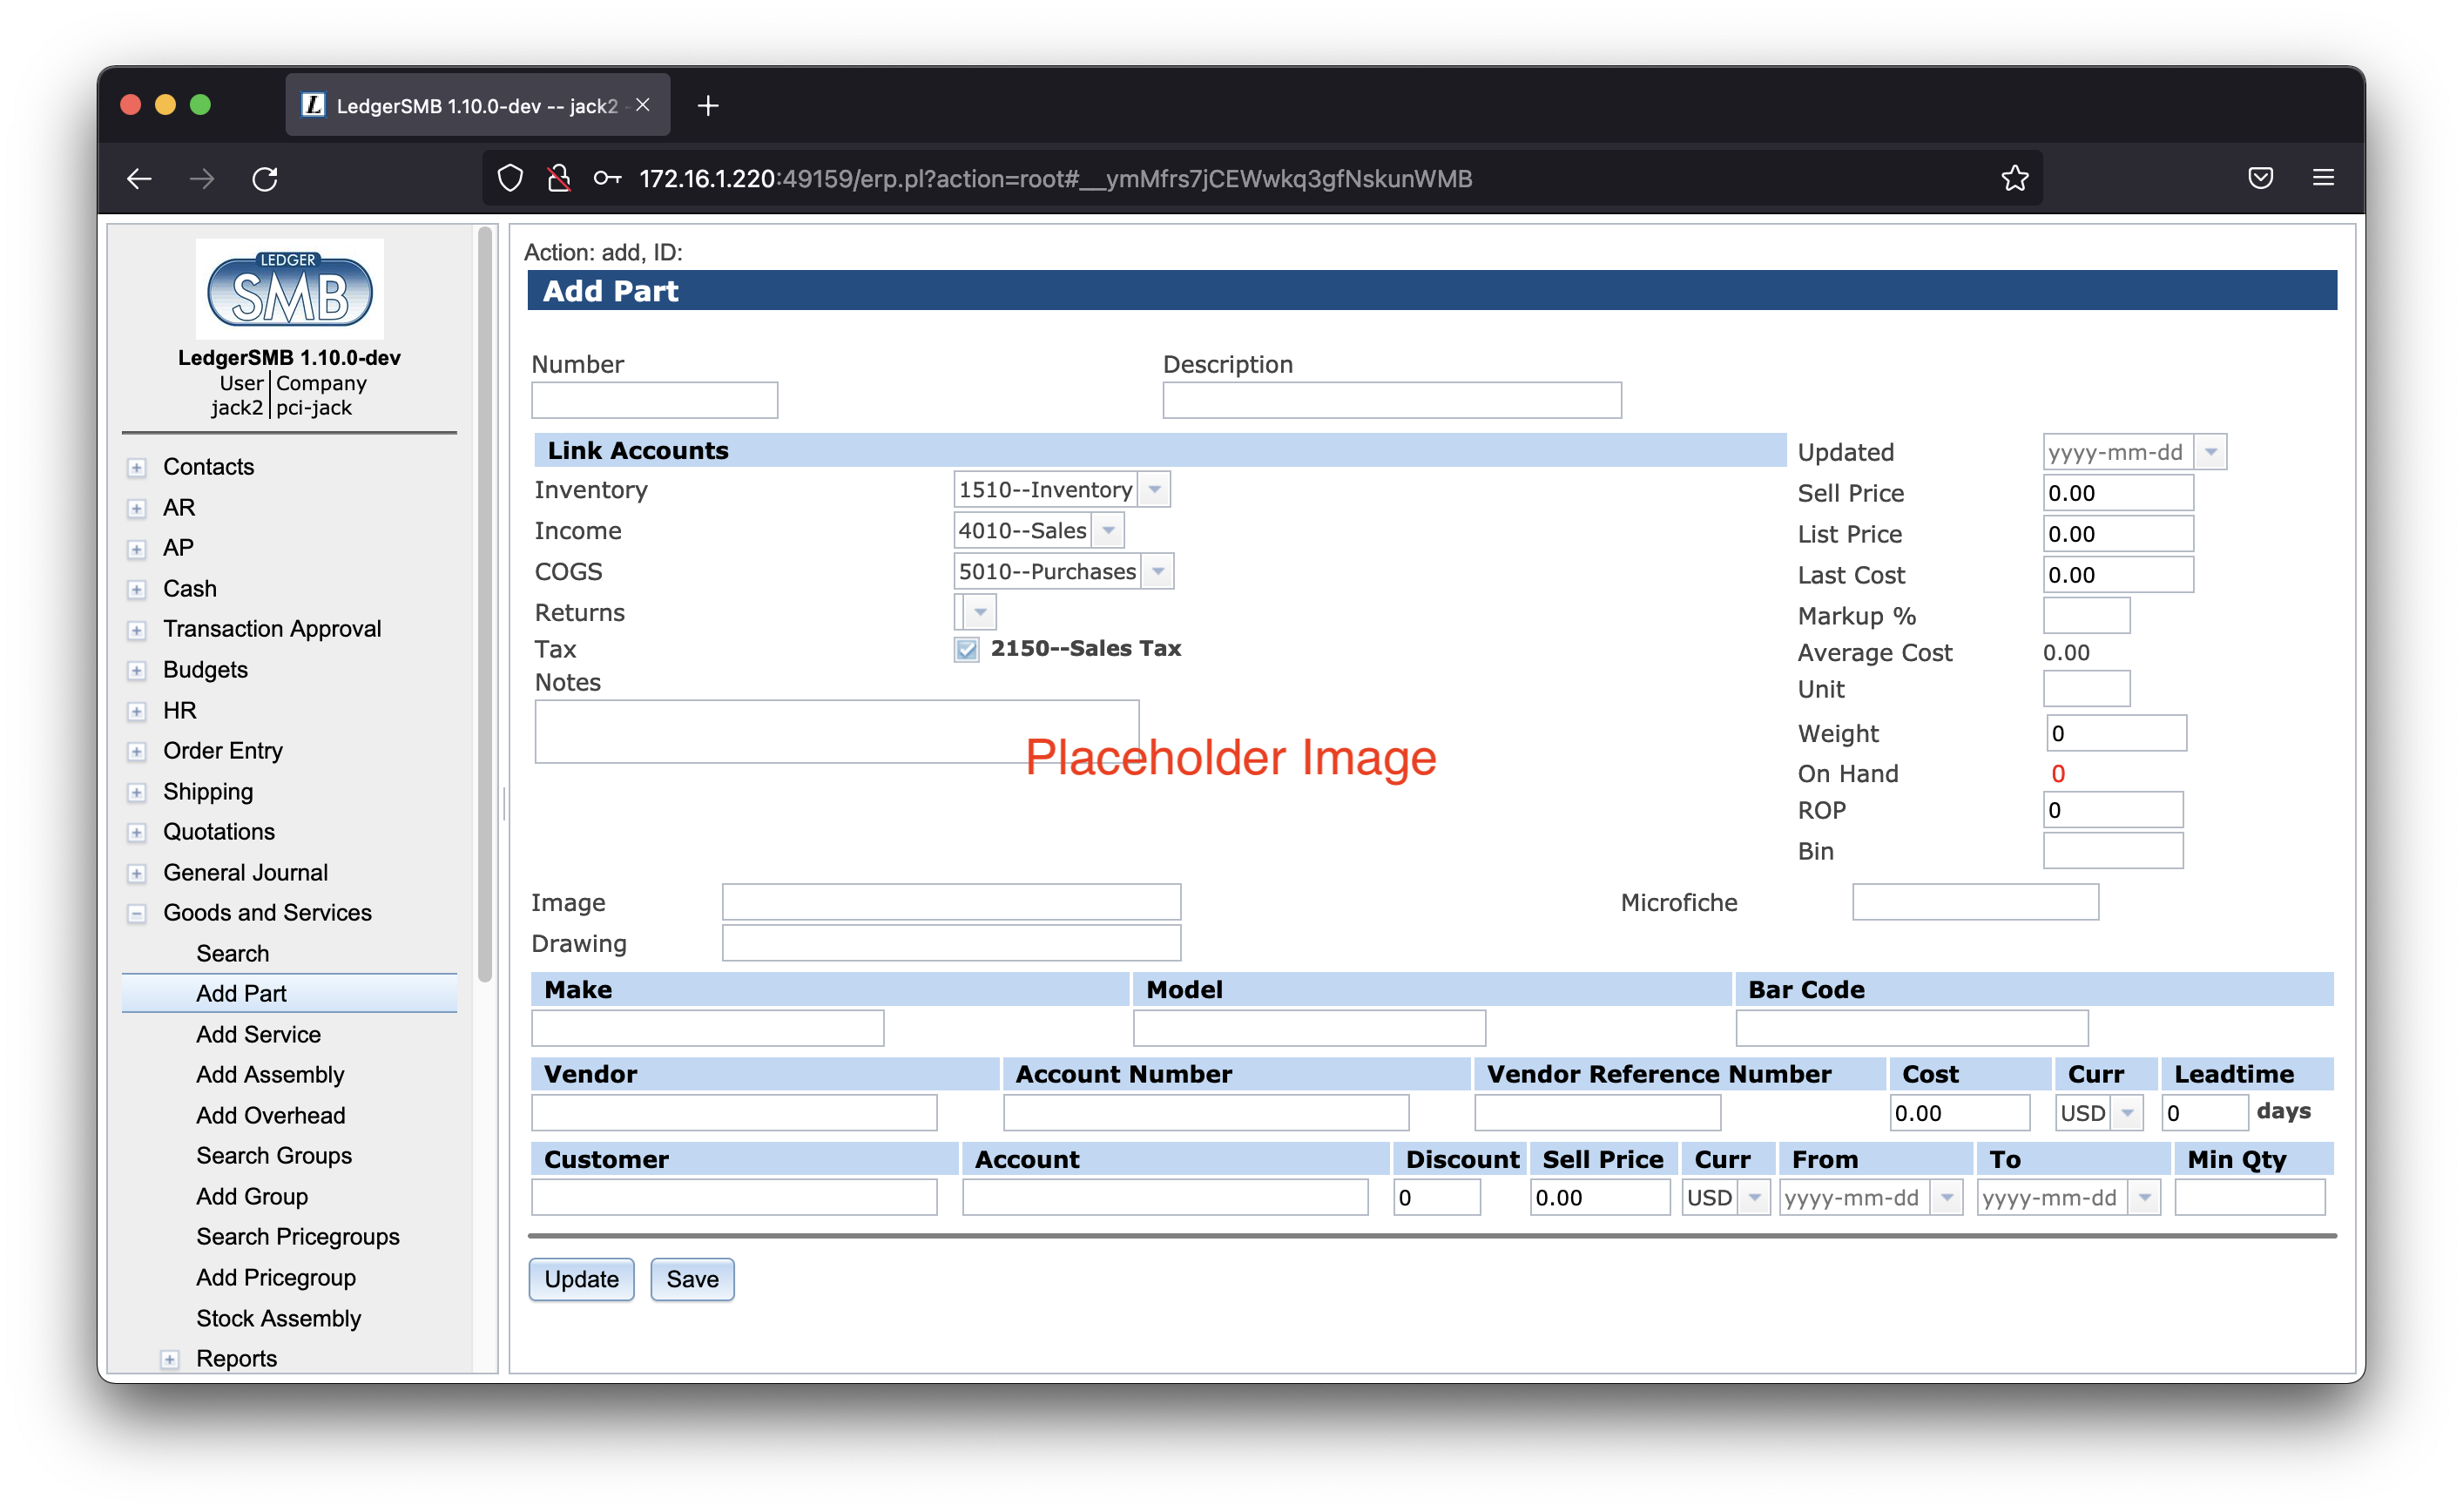
\includegraphics[width=\linewidth]{setup-add-part.png}
        \caption{Add first part}
        \label{fig:setup-add-part}
\end{figure}

Based on his reading from \secref{subsec-products-parts-definition}, Jack decides to enter the hard
drive with the following data:

\begin{tabular}{ll}
Field & Value\\ \hline
Number & \texttt{SAM1TB}\\
Description & \texttt{SAMSUNG 980 PRO 1TB PCIe NVMe Gen4 SSD} \\
Inventory account &  \texttt{1510 - Inventory}\\
Income account &  \texttt{4010 - Sales}\\
COGS account &  \texttt{5010 - Purchases}\\
Sell price &  \texttt{175.00}\\
\\
\end{tabular}

After entering the data Jack clicks \texttt{Save}.

He decides not to include make/model information, drawings or images yet and since
he hasn't entered vendors or customers in his system yet, he decides to leave
those sections blank as well.

\subsection{Combining single-item and ``multi-item pre-packaged'' sales}
\label{subsec-stock-parts-mulit-item}

After having finished setting up the solid state drive, Jack now wants to enter
the memory modules he's going to sell. The problem is that they usually go in pairs,
since that's what the systems consuming them need. However, he expects them to be sold
as single items as well and he wants to be able to set a separate price for those occasions.

From his reading of \secref{subsec-parts-versus-assemblies}, it should be
possible to support this scenario with a small work around\footnote{It's planned to directly
support this use-case in some version higher than 1.3}. From the two solutions available,
he chooses option (b): to create a part and an assembly and regularly restock the assembly
to 0 (zero) in order to remove the stock from the single item.

\section{Defining part groups}
\label{sec-stock-part-groups}

As Jack continues to enter more parts into the system, he wonders how he's going to
look up the parts efficiently later on. Returning his reading to \secref{subsec-products-parts-definition},
he understands that 'part groups' are the solution to that problem. 

He decides to create
the part groups by navigating to:
\begin{quote}
\menupath{Goods and Services \ma Add Group}.
\end{quote}
For each group in the list below Jack enters the group name and clicks \texttt{Save} after each one:

\begin{tabular}{ll}
Field & Value \\ \hline
Group & \texttt{Storage}\\
Group & \texttt{Monitors}\\
Group & \texttt{Input devices}\\
Group & \texttt{Printers}\\
\\
\end{tabular}

After creating these part groups, the ``Group'' drop down appears on the parts entry screen,
allowing him to assign each of his parts to one of these groups.

Since he doesn't expect to be running more than one or two types of CPUs, he decides
not to create a separate group for those and leaves these two parts unassigned.

\section{Defining vendors}
\label{sec-stock-defining-vendors}

Jack selects ``ABC Parts'' to purchase the inventory he needs to run his company. In
order to start buying inventory, ABC Parts needs to be entered as a Vendor to LedgerSMB.

Using the work flow detailed in \secref{sec-business-processes-creating-customers-and-vendors} Jack starts to do so by going through the menu \menupath{Contacts \ma Add Contact \ma Company}.
He fills out the Company creation form by clicking the {\tt Generate control code}
button and adding the data as shown in \figref{fig:vendor-create-1}.

\begin{figure}[h]
\centering
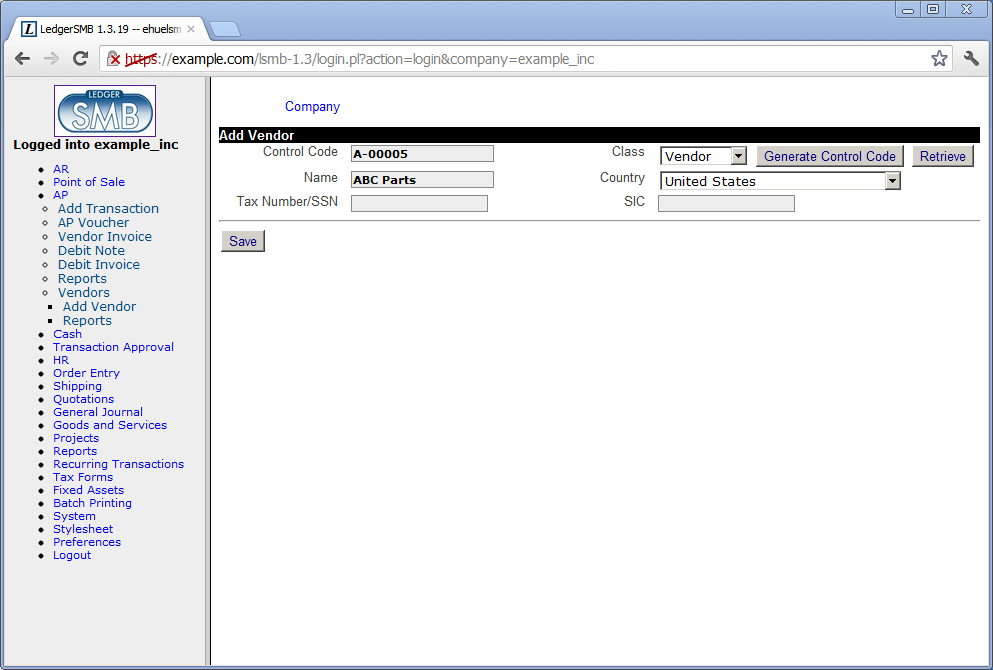
\includegraphics[width=7cm]{bus-vendor-create-2.png}
\caption{Company entry screen}
\label{fig:vendor-create-1}
\end{figure}

After saving the company data, Jack is presented the account data screen which he fills out
as shown in \figref{fig:vendor-create-2}.

\begin{figure}[h]
\centering
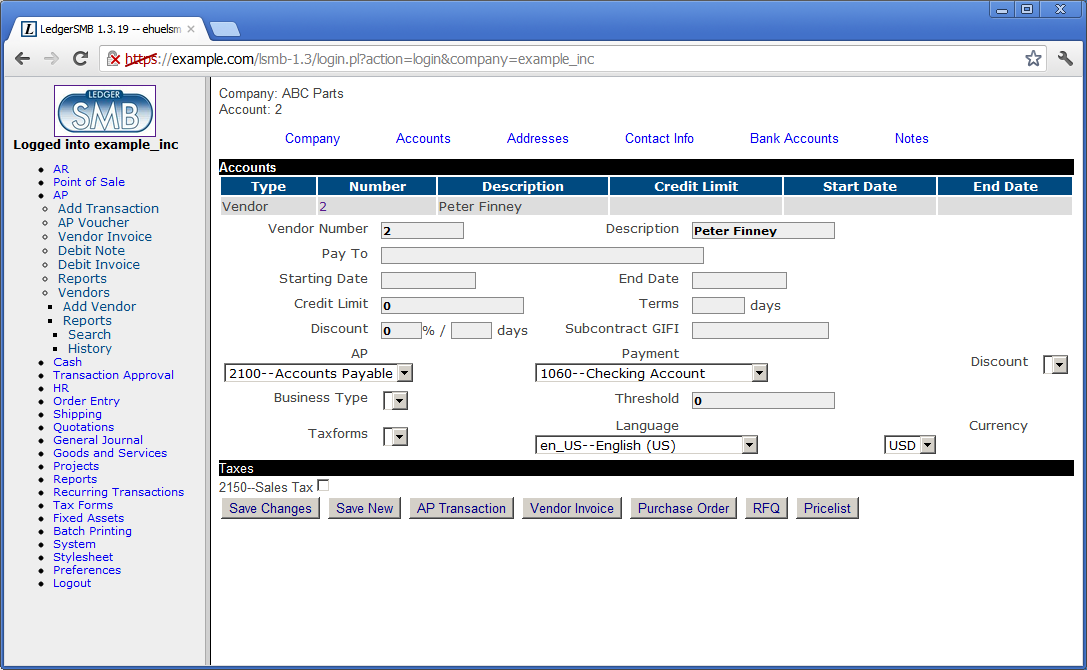
\includegraphics[width=7cm]{bus-vendor-create-3.png}
\caption{Vendor account screen}
\label{fig:vendor-create-2}
\end{figure}

When he's done filling out and saving the form,
he notices the empty ``Discount'' drop down. Reading more about account configuration
check marks in \secref{subsubsec-coa-AR-AP-checkmarks} and going back to the checks on his
chart of accounts (\secref{sec-first-login-coa-check}), he finds he's missing the purchase and
sales discount accounts. He adds two accounts as follows:

\begin{itemize}
\item [4020] Sales discount
\item [5020] Purchase discount
\end{itemize}

After which the page looks like \figref{fig:vendor-create-3}.

\begin{figure}[h]
\centering
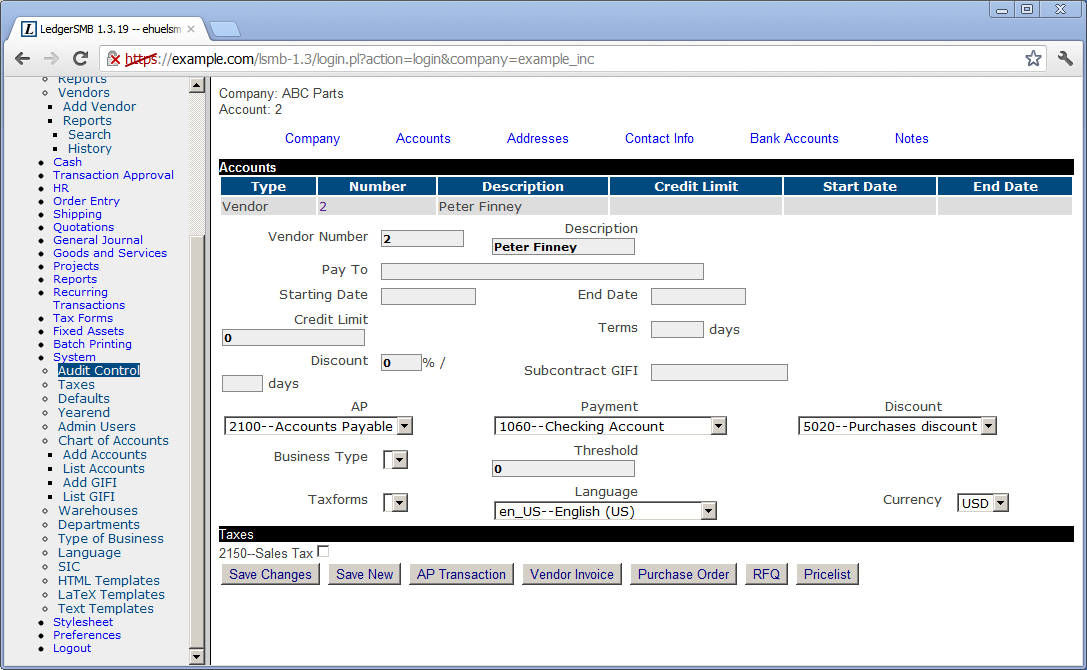
\includegraphics[width=7cm]{bus-vendor-create-4.png}
\caption{Vendor account screen - with purchase discount account}
\label{fig:vendor-create-3}
\end{figure}

Note the top-left corner stating ``Company: ABC Parts'' and ``Account: 2''. The information
entered on the ``Addresses'', ``Contact Info'' and ``Bank Accounts'' tabs will be attached
to the account listed, i.e. account number 2 in this case.

The reader is referred to \secref{sec-business-processes-creating-customers-and-vendors} for a more in-depth
description of the vendor data screens.

\section{Requesting quotations}
\label{sec-stock-request-quotation}

After Jack finishes setting up the parts and vendor information, he decides to use LedgerSMB to draw
up a list of items he wants to order from this company. To do so he follows the menu path
\menupath{Quotations \ma RFQ} which opens up a screen (shown
in \figref{fig:rfq-entry-screen}) for entering a new \gls{rfq} .

\begin{figure}[h]
\centering
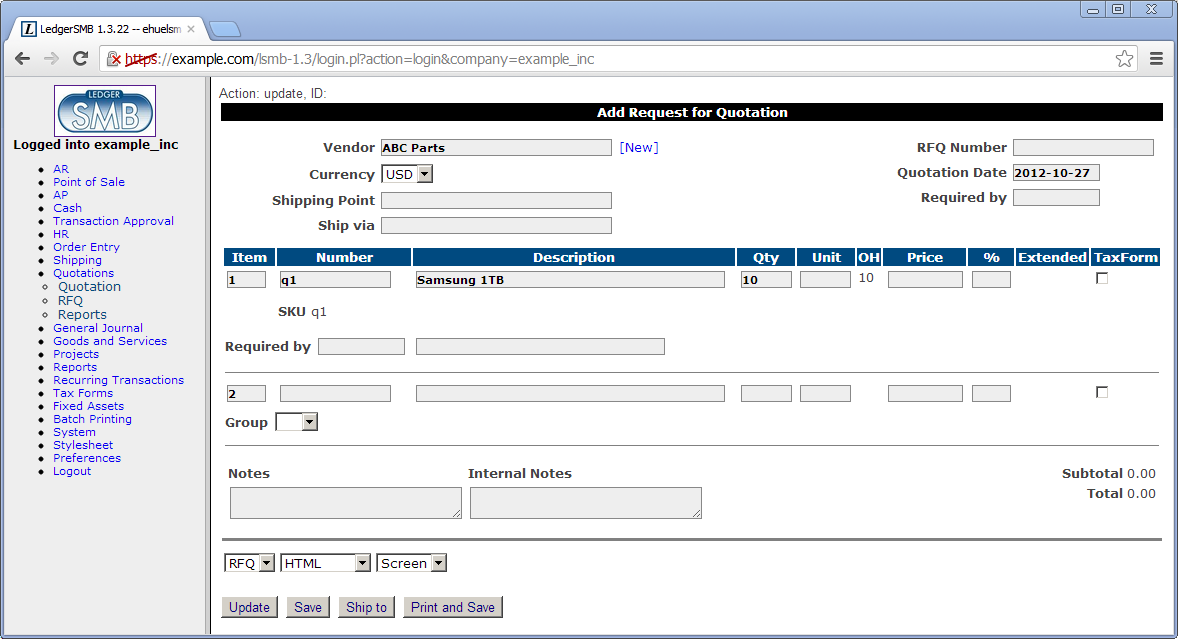
\includegraphics[width=7cm]{rfq-entry-screen.png}
\caption{RFQ entry screen}
\label{fig:bus-rfq-entry-screen}
\end{figure}

\begin{quotation}
\textbf{Remark} Note that the \gls{rfq} entry screen contains prices; this is misleading
at least: the printed output to be sent to the vendor does not. The fact that this screen
allows entry of prices could be considered a bug.
\end{quotation}

After filling out the form in accordance with the description in \secref{sec-business-processes-quotations-creation},
Jack expedites his \gls{rfq} to his vendor through e-mail by clicking the ``E-mail'' button. He finds
himself in the screen shown in \figref{fig:rfq-email-screen}.

The From field of the e-mail to be sent out will be filled using the ``Default From'' setting documented
in \secref{subsec-company-config-defaults}. The other address fields can be entered by the user and may be readily
populated if the customer account has the right contact info items attached: if there are Email, Cc and/or
Bcc contact items set up, those will be used to fill these fields.

At the bottom there are three selection lists. The first allows selection of the format used to send the
\gls{rfq}. Available options are HTML, CSV, Postscript (PS) and PDF. The last two require Postscript and PDF
support to be correctly set up. The last selection list selects the language to be used for the
\gls{rfq}. If no value is selected the system default language is used.

\begin{figure}[h]
\centering
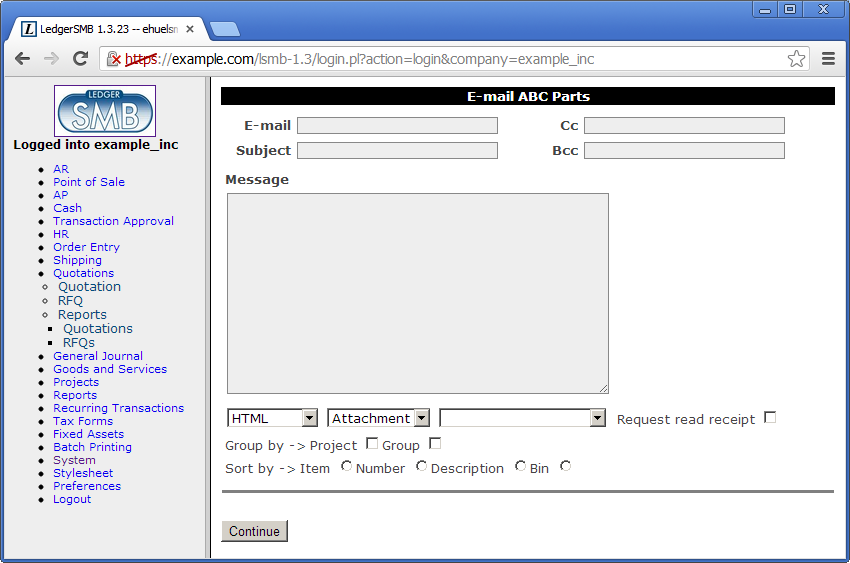
\includegraphics[width=7cm]{rfq-email-screen.png}
\caption{RFQ e-mail screen}
\label{fig:rfq-email-screen}
\end{figure}

For more detail, the reader is referred to \secref{subsec-business-processes-quotations-sending-email}.


\section{Following up on a quotation}
\label{sec-stock-quotation-followup}

Jack's vendor (ABC Parts) sends him a quotation in response to his \gls{rfq}. Jack and his vendor
can go back and forth a few times until Jack likes the offer he's getting, but for the sake of
argument let's assume this is the final quotation.

Since Jack likes the offer, he wants to place an order with his vendor. To do so he looks up the
\gls{rfq} he sent to the vendor using the menu path \menupath{Quotations \ma Reports \ma Search}.
The screen shows additional buttons now that it shows a saved RFQ.


\begin{figure}[h]
\centering
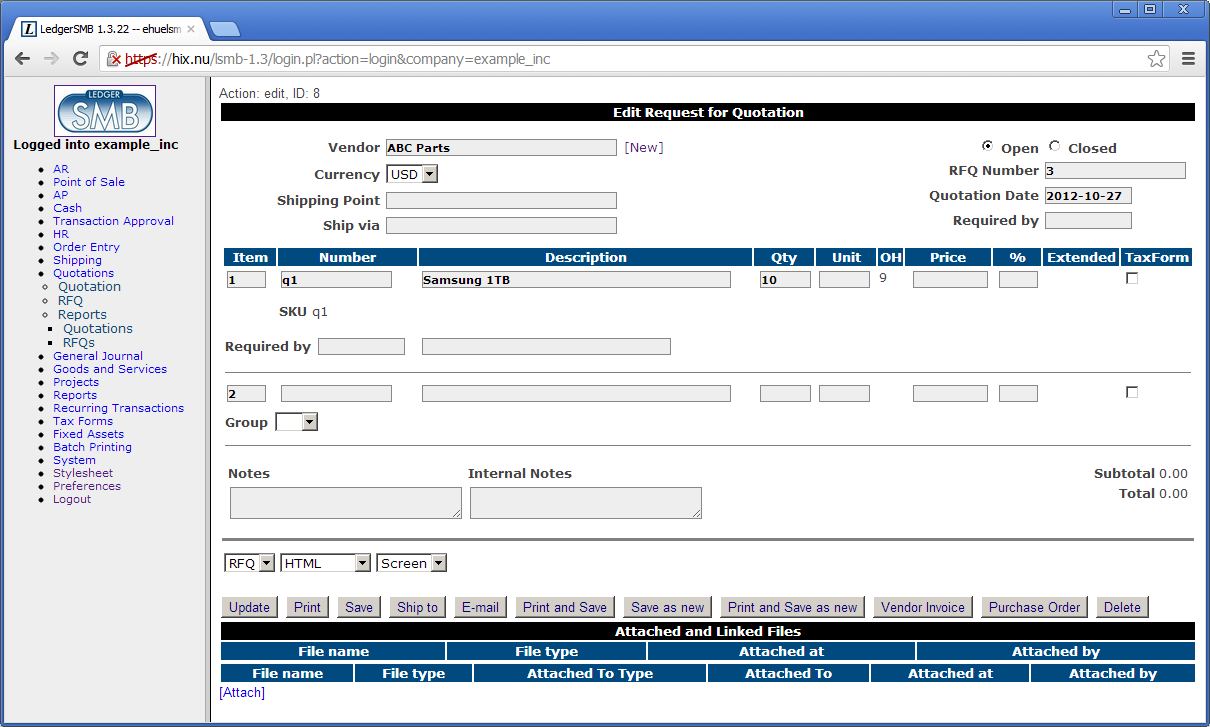
\includegraphics[width=7cm]{rfq-edit-screen.png}
\caption{RFQ entry screen}
\label{fig:bus-rfq-edit-screen}
\end{figure}

Jack clicks the ``Purchase Order'' button which creates a new order from the data in the RFQ.
He completes it
by entering the prices his vendor has quoted and by modifying it to be in accordance with the
quotation. See \secref{sec-business-processes-orders-creation-from-quotations} for more
detail on the order entry screen. When finished he saves the order and mails it to
ABC Parts just like he mailed the \gls{rfq} in the previous section.

\figref{fig:purchase-order-screen} shows the screen of a saved purchase order.

\section{Receiving ordered items}
\label{sec-stock-receiving}

Having ordered his inventory, the vendor starts shipping. There's too much to ship at once
so the vendor ships the goods in batches: every week he ships what's available at the end
of that week - he needed to order some of the products with the manufacturer.

LedgerSMB helps Jack keep track to see if he has received everything he has ordered and
that he's not receiving too much. Jack goes through the menus \menupath{Shipping \ma Receive}.
In the search screen, he fills the vendor name (ABC Parts) and clicks ``Continue'' to be listed
all open orders from ABC Parts. By clicking on the order number, the ``Receive Merchandise'' screen
opens as presented in \figref{fig:order-receive-screen}. This allows Jack to handle the incoming
shipment. LedgerSMB will automatically update inventory based on the amounts entered as received
\footnote{To resolve problems in the inventory tracking parts of LedgerSMB (inherited from
before the fork), a significant change has been implemented in 1.3.31: inventory changes won't
be recorded until invoices have been posted.
}.

\begin{figure}[h]
\centering
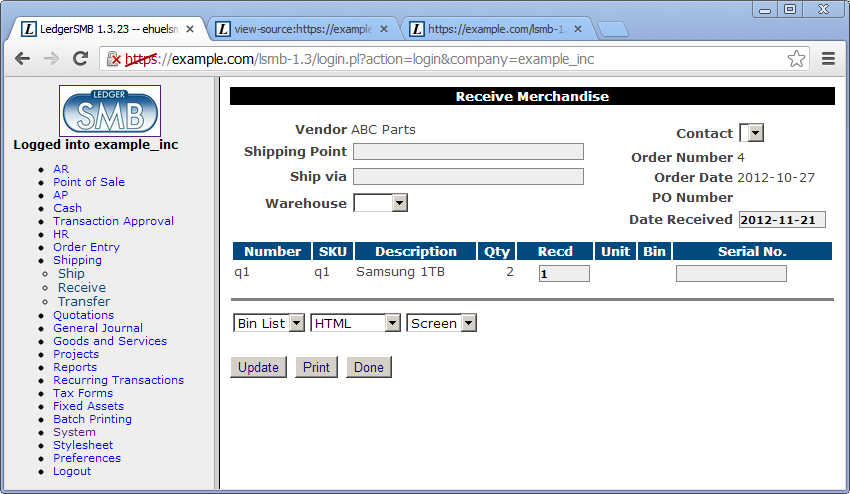
\includegraphics[width=7cm]{order-receive-screen.png}
\caption{Order receipt entry screen}
\label{fig:order-receive-screen}
\end{figure}

\section{Receiving an invoice}
\label{sec-stock-invoice}

\section{Paying an invoice}
\label{sec-stock-payment}



\chapter{Ramping up to the first sale}
\label{cha-ramping-up-to-the-first-sale}

\section{Sending out a quote} 
\label{sec-sending-a-quote}

\section{Sending out a sales order}
\label{sec-sending-a-sales-order}



\chapter{Shipping sales}
\label{cha-shipping-sales}



\chapter{Invoicing}
\label{cha-starting-invoicing}

\section{Handling sales taxes}
\label{sec-invoicing-sales-tax}

\subsection{Invoices with taxes included}
\label{subsec-sales-tax-included}

\subsection{Invoices with explicit tax amounts}
\label{subsec-sales-tax-explicit-amount}

\section{Invoice Editing}
\label{sec-invoicing-editing}

Posted invoices only have 2 fields that can be edited:
\begin{enumerate}
\item Internal notes field
\item Sales person - The Sales Person drop-down is only shown if there are sales people. Sales People are created through Employees and checking the Sales check-mark.
\end{enumerate}
After editing, click the  \texttt{Save Info} button to save the changes.

\chapter{Collecting sales invoice payments}
\label{cha-starting-sales-customer-payments}

\section{Customer payments}
\label{sec-starting-sales-customer-payments}

\section{Customer payment mismatch}
\label{sec-starting-sales-payment-mismatch}

\subsection{Choosing between pardoning and registering underpayment}
\label{subsec-sales-payment-mismatch}

\subsection{Large ones, as in partial payments or largish under/over payments}
\label{subsec-sales-payment-partial}

\subsection{Pardoning small mismatches}
\label{subsec-sales-payment-pardoning}



\chapter{Paying vendor invoices}
\label{cha-starting-vendor-payments}

\section{Handling vendors who match amounts to exact invoices}
\label{sec-vendor-invoice-exact-match}

\section{Handling vendors with running balances}
\label{sec-vendor-invoice-running-balance}

\section{Handling bounced checks}
\label{sec-vendor-invoice-bounced-checks}

\subsection{Voiding checks to undo payments of vendor invoices
 relating to bounced checks}



\chapter{Monitoring arrears}
\label{cha-starting-monitoring-arrears}

\section{Handling interest on arrears}
\label{sec-monitoring-interest-on-arrears}



\chapter{Branching out: services}
\label{cha-starting-branch-to-services}

\section{Creation / assignment to different accounts}
\label{sec-starting-services-assignment}

\section{Recording service hours}
\label{sec-starting-services-writing-hours}

\section{Customer approval on service hours}
\label{sec-starting-services-hours-customer-approval}

\section{Invoicing services}
\label{sec-starting-services-invoicing}

\chapter{Branching out II: service subscriptions}
\label{cha-starting-services-subscriptions}

